\documentclass[10pt, oneside]{article} 
\usepackage{amsmath, amsthm, amssymb, calrsfs, wasysym, verbatim, bbm, color, graphics, geometry, esint, float}


\geometry{tmargin=.75in, bmargin=.75in, lmargin=.75in, rmargin = .75in}  

\newcommand{\bbR}{\mathbb{R}}
\newcommand{\bbC}{\mathbb{C}}
\newcommand{\bbZ}{\mathbb{Z}}
\newcommand{\bbN}{\mathbb{N}}
\newcommand{\bbQ}{\mathbb{Q}}
\newcommand{\Cdot}{\boldsymbol{\cdot}}
\newcommand{\scA}{\mathscr{A}}
\newcommand{\curl}{\text{curl}}

\theoremstyle{definition}
\newtheorem{exmp}{Example}[section]
\newtheorem{thm}{Theorem}
\newtheorem{defn}{Definition}
\newtheorem{prop}{Proposition}
\newtheorem{conv}{Convention}
\newtheorem{rem}{Remark}
\newtheorem{lem}{Lemma}
\newtheorem{cor}{Corollary}
% Copyright 2021 Paolo Adajar (padajar.com, paoloadajar@mit.edu)
% 
% Permission is hereby granted, free of charge, to any person obtaining a copy of this software and associated documentation files (the "Software"), to deal in the Software without restriction, including without limitation the rights to use, copy, modify, merge, publish, distribute, sublicense, and/or sell copies of the Software, and to permit persons to whom the Software is furnished to do so, subject to the following conditions:
%
% The above copyright notice and this permission notice shall be included in all copies or substantial portions of the Software.
% 
% THE SOFTWARE IS PROVIDED "AS IS", WITHOUT WARRANTY OF ANY KIND, EXPRESS OR IMPLIED, INCLUDING BUT NOT LIMITED TO THE WARRANTIES OF MERCHANTABILITY, FITNESS FOR A PARTICULAR PURPOSE AND NONINFRINGEMENT. IN NO EVENT SHALL THE AUTHORS OR COPYRIGHT HOLDERS BE LIABLE FOR ANY CLAIM, DAMAGES OR OTHER LIABILITY, WHETHER IN AN ACTION OF CONTRACT, TORT OR OTHERWISE, ARISING FROM, OUT OF OR IN CONNECTION WITH THE SOFTWARE OR THE USE OR OTHER DEALINGS IN THE SOFTWARE.

\usepackage{fullpage}
\usepackage{enumitem}
\usepackage{amsfonts, amssymb, amsmath,amsthm}
\usepackage{mathtools}
\usepackage[pdftex, pdfauthor={\name}, pdftitle={\classnum~\assignment}]{hyperref}
\usepackage[dvipsnames]{xcolor}
\usepackage{bbm}
\usepackage{graphicx}
\usepackage{mathrsfs}
\usepackage{pdfpages}
\usepackage{tabularx}
\usepackage{pdflscape}
\usepackage{makecell}
\usepackage{booktabs}
\usepackage{natbib}
\usepackage{caption}
\usepackage{subcaption}
\usepackage{physics}
\usepackage[many]{tcolorbox}
\usepackage{version}
\usepackage{ifthen}
\usepackage{cancel}
\usepackage{listings}
\usepackage{courier}

\usepackage{tikz}
\usepackage{istgame}

\hypersetup{
	colorlinks=true,
	linkcolor=blue,
	filecolor=magenta,
	urlcolor=blue,
}

\setlength{\parindent}{0mm}
\setlength{\parskip}{2mm}

\setlist[enumerate]{label=({\alph*})}
\setlist[enumerate, 2]{label=({\roman*})}

\allowdisplaybreaks[1]

\newcommand{\psetheader}{
	\ifthenelse{\isundefined{\collaborators}}{
		\begin{center}
			{\setlength{\parindent}{0cm} \setlength{\parskip}{0mm}
				
				{\textbf{\classnum~\semester:~\assignment} \hfill \name}
				
				\subject \hfill \href{mailto:\email}{\tt \email}
				
				Instructor(s):~\instructors \hfill Due Date:~\duedate	
				
				\hrulefill}
		\end{center}
	}{
		\begin{center}
			{\setlength{\parindent}{0cm} \setlength{\parskip}{0mm}
				
				{\textbf{\classnum~\semester:~\assignment} \hfill \name\footnote{Collaborator(s): \collaborators}}
				
				\subject \hfill \href{mailto:\email}{\tt \email}
				
				Instructor(s):~\instructors \hfill Due Date:~\duedate	
				
				\hrulefill}
		\end{center}
	}
}

\renewcommand{\thepage}{\classnum~\assignment \hfill \arabic{page}}

\makeatletter
\def\points{\@ifnextchar[{\@with}{\@without}}
\def\@with[#1]#2{{\ifthenelse{\equal{#2}{1}}{{[1 point, #1]}}{{[#2 points, #1]}}}}
\def\@without#1{\ifthenelse{\equal{#1}{1}}{{[1 point]}}{{[#1 points]}}}
\makeatother

\newtheoremstyle{theorem-custom}%
{}{}%
{}{}%
{\itshape}{.}%
{ }%
{\thmname{#1}\thmnumber{ #2}\thmnote{ (#3)}}

\theoremstyle{theorem-custom}

\newtheorem{theorem}{Theorem}
\newtheorem{lemma}[theorem]{Lemma}
\newtheorem{example}[theorem]{Example}

\newenvironment{problem}[1]{\color{black} #1}{}

\newenvironment{solution}{%
	\leavevmode\begin{tcolorbox}[breakable, colback=green!5!white,colframe=green!75!black, enhanced jigsaw] \proof[\scshape Solution:] \setlength{\parskip}{2mm}%
	}{\renewcommand{\qedsymbol}{$\blacksquare$} \endproof \end{tcolorbox}}

\newenvironment{reflection}{\begin{tcolorbox}[breakable, colback=black!8!white,colframe=black!60!white, enhanced jigsaw, parbox = false]\textsc{Reflections:}}{\end{tcolorbox}}

\newcommand{\qedh}{\renewcommand{\qedsymbol}{$\blacksquare$}\qedhere}

\definecolor{mygreen}{rgb}{0,0.6,0}
\definecolor{mygray}{rgb}{0.5,0.5,0.5}
\definecolor{mymauve}{rgb}{0.58,0,0.82}

% from https://github.com/satejsoman/stata-lstlisting
% language definition
\lstdefinelanguage{Stata}{
	% System commands
	morekeywords=[1]{regress, reg, summarize, sum, display, di, generate, gen, bysort, use, import, delimited, predict, quietly, probit, margins, test},
	% Reserved words
	morekeywords=[2]{aggregate, array, boolean, break, byte, case, catch, class, colvector, complex, const, continue, default, delegate, delete, do, double, else, eltypedef, end, enum, explicit, export, external, float, for, friend, function, global, goto, if, inline, int, local, long, mata, matrix, namespace, new, numeric, NULL, operator, orgtypedef, pointer, polymorphic, pragma, private, protected, public, quad, real, return, rowvector, scalar, short, signed, static, strL, string, struct, super, switch, template, this, throw, transmorphic, try, typedef, typename, union, unsigned, using, vector, version, virtual, void, volatile, while,},
	% Keywords
	morekeywords=[3]{forvalues, foreach, set},
	% Date and time functions
	morekeywords=[4]{bofd, Cdhms, Chms, Clock, clock, Cmdyhms, Cofc, cofC, Cofd, cofd, daily, date, day, dhms, dofb, dofC, dofc, dofh, dofm, dofq, dofw, dofy, dow, doy, halfyear, halfyearly, hh, hhC, hms, hofd, hours, mdy, mdyhms, minutes, mm, mmC, mofd, month, monthly, msofhours, msofminutes, msofseconds, qofd, quarter, quarterly, seconds, ss, ssC, tC, tc, td, th, tm, tq, tw, week, weekly, wofd, year, yearly, yh, ym, yofd, yq, yw,},
	% Mathematical functions
	morekeywords=[5]{abs, ceil, cloglog, comb, digamma, exp, expm1, floor, int, invcloglog, invlogit, ln, ln1m, ln, ln1p, ln, lnfactorial, lngamma, log, log10, log1m, log1p, logit, max, min, mod, reldif, round, sign, sqrt, sum, trigamma, trunc,},
	% Matrix functions
	morekeywords=[6]{cholesky, coleqnumb, colnfreeparms, colnumb, colsof, corr, det, diag, diag0cnt, el, get, hadamard, I, inv, invsym, issymmetric, J, matmissing, matuniform, mreldif, nullmat, roweqnumb, rownfreeparms, rownumb, rowsof, sweep, trace, vec, vecdiag, },
	% Programming functions
	morekeywords=[7]{autocode, byteorder, c, _caller, chop, abs, clip, cond, e, fileexists, fileread, filereaderror, filewrite, float, fmtwidth, has_eprop, inlist, inrange, irecode, matrix, maxbyte, maxdouble, maxfloat, maxint, maxlong, mi, minbyte, mindouble, minfloat, minint, minlong, missing, r, recode, replay, return, s, scalar, smallestdouble,},
	% Random-number functions
	morekeywords=[8]{rbeta, rbinomial, rcauchy, rchi2, rexponential, rgamma, rhypergeometric, rigaussian, rlaplace, rlogistic, rnbinomial, rnormal, rpoisson, rt, runiform, runiformint, rweibull, rweibullph,},
	% Selecting time-span functions
	morekeywords=[9]{tin, twithin,},
	% Statistical functions
	morekeywords=[10]{betaden, binomial, binomialp, binomialtail, binormal, cauchy, cauchyden, cauchytail, chi2, chi2den, chi2tail, dgammapda, dgammapdada, dgammapdadx, dgammapdx, dgammapdxdx, dunnettprob, exponential, exponentialden, exponentialtail, F, Fden, Ftail, gammaden, gammap, gammaptail, hypergeometric, hypergeometricp, ibeta, ibetatail, igaussian, igaussianden, igaussiantail, invbinomial, invbinomialtail, invcauchy, invcauchytail, invchi2, invchi2tail, invdunnettprob, invexponential, invexponentialtail, invF, invFtail, invgammap, invgammaptail, invibeta, invibetatail, invigaussian, invigaussiantail, invlaplace, invlaplacetail, invlogistic, invlogistictail, invnbinomial, invnbinomialtail, invnchi2, invnF, invnFtail, invnibeta, invnormal, invnt, invnttail, invpoisson, invpoissontail, invt, invttail, invtukeyprob, invweibull, invweibullph, invweibullphtail, invweibulltail, laplace, laplaceden, laplacetail, lncauchyden, lnigammaden, lnigaussianden, lniwishartden, lnlaplaceden, lnmvnormalden, lnnormal, lnnormalden, lnwishartden, logistic, logisticden, logistictail, nbetaden, nbinomial, nbinomialp, nbinomialtail, nchi2, nchi2den, nchi2tail, nF, nFden, nFtail, nibeta, normal, normalden, npnchi2, npnF, npnt, nt, ntden, nttail, poisson, poissonp, poissontail, t, tden, ttail, tukeyprob, weibull, weibullden, weibullph, weibullphden, weibullphtail, weibulltail,},
	% String functions 
	morekeywords=[11]{abbrev, char, collatorlocale, collatorversion, indexnot, plural, plural, real, regexm, regexr, regexs, soundex, soundex_nara, strcat, strdup, string, strofreal, string, strofreal, stritrim, strlen, strlower, strltrim, strmatch, strofreal, strofreal, strpos, strproper, strreverse, strrpos, strrtrim, strtoname, strtrim, strupper, subinstr, subinword, substr, tobytes, uchar, udstrlen, udsubstr, uisdigit, uisletter, ustrcompare, ustrcompareex, ustrfix, ustrfrom, ustrinvalidcnt, ustrleft, ustrlen, ustrlower, ustrltrim, ustrnormalize, ustrpos, ustrregexm, ustrregexra, ustrregexrf, ustrregexs, ustrreverse, ustrright, ustrrpos, ustrrtrim, ustrsortkey, ustrsortkeyex, ustrtitle, ustrto, ustrtohex, ustrtoname, ustrtrim, ustrunescape, ustrupper, ustrword, ustrwordcount, usubinstr, usubstr, word, wordbreaklocale, worcount,},
	% Trig functions
	morekeywords=[12]{acos, acosh, asin, asinh, atan, atanh, cos, cosh, sin, sinh, tan, tanh,},
	morecomment=[l]{//},
	% morecomment=[l]{*},  // `*` maybe used as multiply operator. So use `//` as line comment.
	morecomment=[s]{/*}{*/},
	% The following is used by macros, like `lags'.
	morestring=[b]{`}{'},
	% morestring=[d]{'},
	morestring=[b]",
	morestring=[d]",
	% morestring=[d]{\\`},
	% morestring=[b]{'},
	sensitive=true,
}

\lstset{ 
	backgroundcolor=\color{white},   % choose the background color; you must add \usepackage{color} or \usepackage{xcolor}; should come as last argument
	basicstyle=\footnotesize\ttfamily,        % the size of the fonts that are used for the code
	breakatwhitespace=false,         % sets if automatic breaks should only happen at whitespace
	breaklines=true,                 % sets automatic line breaking
	captionpos=b,                    % sets the caption-position to bottom
	commentstyle=\color{mygreen},    % comment style
	deletekeywords={...},            % if you want to delete keywords from the given language
	escapeinside={\%*}{*)},          % if you want to add LaTeX within your code
	extendedchars=true,              % lets you use non-ASCII characters; for 8-bits encodings only, does not work with UTF-8
	firstnumber=0,                % start line enumeration with line 1000
	frame=single,	                   % adds a frame around the code
	keepspaces=true,                 % keeps spaces in text, useful for keeping indentation of code (possibly needs columns=flexible)
	keywordstyle=\color{blue},       % keyword style
	language=Octave,                 % the language of the code
	morekeywords={*,...},            % if you want to add more keywords to the set
	numbers=left,                    % where to put the line-numbers; possible values are (none, left, right)
	numbersep=5pt,                   % how far the line-numbers are from the code
	numberstyle=\tiny\color{mygray}, % the style that is used for the line-numbers
	rulecolor=\color{black},         % if not set, the frame-color may be changed on line-breaks within not-black text (e.g. comments (green here))
	showspaces=false,                % show spaces everywhere adding particular underscores; it overrides 'showstringspaces'
	showstringspaces=false,          % underline spaces within strings only
	showtabs=false,                  % show tabs within strings adding particular underscores
	stepnumber=2,                    % the step between two line-numbers. If it's 1, each line will be numbered
	stringstyle=\color{mymauve},     % string literal style
	tabsize=2,	                   % sets default tabsize to 2 spaces
%	title=\lstname,                   % show the filename of files included with \lstinputlisting; also try caption instead of title
	xleftmargin=0.25cm
}



\title{UChicago Honors Analysis Notes: 20800}
\author{Notes by Agustín Esteva, Lectures by Panagiotis E. Souganidis, Books by Walter Rudin, Haim Brezis}
\date{Academic Year 2024-2025}

\begin{document}

\maketitle
\tableofcontents

\vspace{.25in}


\newpage
\section{Lectures}

\subsection{Monday, Jan 6: The Stieltjes Integral}
We begin by constructing the integral. Assume $f: [a,b]\to \bbR$ is continuous and $\alpha: [a,b]\to \bbR$ is monotonic. 
\begin{rem}
    The monotonicity assumption is made in order to control the variation of $\alpha,$ as monotonic functions can only have jump discontinuities (and countably many, prove this if you want, I don't care). Moreover, $\alpha$ is usually taken to be increasing to be consistent with all the upper sum being greater than the lower sum deal. 
\end{rem}
Suppose $P$ partitions $[a,b]$ into $\{x_0, x_1, \dots, x_n\},$ then we say that the upper sum is
\[U(P, f, \alpha) = \sum_{i=1}^n M_i (\alpha(x_i) - \alpha(x_{i-1})),\] where $M_i$ is defined as \[M_i = \sup_{x\in (x_{i-1}, x_i]}f(x).\] The lower sum $L(P, f, \alpha)$ is similarly defined. We say the upper integral of $f$ with respect to $\alpha$ is 
\[\overline{\int_a^b}f(x)d\alpha(x) = \inf_P  U(P, f, \alpha).\] We similarly define the lower integral.
We say $f\in \mathcal{R}(\alpha),$ or $f$ is \textit{Riemann-Stieltjes integrable with respect to $\alpha$} if 
\[\underline{\int_a^b}f(x)d\alpha(x) = \overline{\int_a^b}f(x)d\alpha(x).\]
\begin{defn}
    We denote the \textit{Stietljes integral} with
    \[\int_a^b f(x) d(\alpha(x)) ``=" \int_a^bf d\alpha.\]
\end{defn}
\begin{defn}
    We say that $P^\ast$ is a \textit{refinement} of $P$ if $P\subset P^\ast.$
\end{defn}
\begin{prop}
    Suppose $P^\ast$ is a refinement of $P,$ then 
    \[U(P^\ast, f, \alpha) \leq U(P, f, \alpha), \qquad L(P^\ast, f, \alpha) \geq L(P, f, \alpha).\]
\end{prop}
We did not prove this. If I have time after I will go crazy. It is an induction proof.
\begin{thm}
    Suppose $f$ is bounded and satisfies the usual conditions w $\alpha,$ then $f\in \mathcal{R}(\alpha)$ if and only if for all $\epsilon>0,$ there exists a partition $P$ such that 
    \[U(P, f, \alpha) - L(P, f, \alpha) < \epsilon.\]
\end{thm}
The proof for one direction is trivial, the other way is an $\frac{\epsilon}{2}$ proof.
\begin{rem}
    We can approximate the integral by 
    \[\int_a^b f d\alpha = \sum_{i=1}^n f(t_i)\Delta \alpha_i, \qquad t_i \in [x_{i-1}, x_i].\]
\end{rem}
\begin{prop}
    The Stieltjes integral satisfies linearity in both $f$ and $\alpha.$
\end{prop}
Proofs follow immediately from the construction.

\begin{thm}
    If $f\in C([a,b]),$ then $f\in \mathcal{R}(\alpha).$ 
\end{thm}
\begin{proof}
    Since $f$ is continuous on $[a,b],$ then $f$ is uniformly continuous on $[a,b],$ and so there exists a $\delta>0$ such that if $|s-t|< \delta$ with $s,t \in [a,b],$ then $|f(s) - f(t)|< \frac{\epsilon}{\alpha(b)-\alpha(a)}.$ Let $P$ be a partition of $[a,b]$ with $||P||< \delta.$ Then we have that telescoping the sum,
    \[U(P,f\alpha) - L(P, f, \alpha) = \sum_{i=1}^n (M_i - m_i)\Delta \alpha_i < \epsilon.\]
\end{proof}

\begin{thm}
    If $f$ is monotone and $\alpha$ is continuous, then $f\in \mathcal{R}(\alpha).$ 
\end{thm}
\begin{proof}
    By assumptions, we can choose a partition such that 
    \[\Delta \alpha_i = \frac{\alpha(b) - \alpha(a)}{n},\] where $n$ is really large. Thus, we have that by the monotonicity of $f,$
    \[U(P,f\alpha) - L(P, f, \alpha) = \sum_{i=1}^n (M_i - m_i)\Delta \alpha_i = \sum_{i=1}^n (f(x_i) - f(x_{i-1}))\Delta \alpha_i < f(b) - f(a)\frac{\alpha(b) - \alpha(a)}{n} < \epsilon.\]
\end{proof}

\begin{thm}
    If $f$ is bounded with finitely many discontinuity points and $\alpha$ is continuous at the points of discontinuity of $f,$ then $f \in \mathcal{R}(\alpha).$
\end{thm}
\begin{proof}
    Let $D$ denote the set of discontinuity points of $\alpha.$ Partition $P$ such that each interval contains one discontinuity each. Then either $x \in D$ for all $x \in [x_{i-1}, x_i]$ or $x\notin D$ for some $x \in [x_{i-1}, x_i].$ If the former, then we can bound the sum by $\frac{\epsilon}{2}$ using Theorem 2. If the latter, then since we know $f$ is bounded, we know that for that interval, $M_i - m_i \leq 2K,$ where $K$ is the max of the magnitude of the upper and lower bounds of $f.$ Since $\alpha$ is continuous at the point of discontinuity, then we can bound $\alpha(x_i) - \alpha(x_{i-1})$ by whatever we want.
    \[U(P,f, \alpha) - L(P, f, \alpha) = \sum_{i=1}^n (M_i - m_i)\Delta \alpha_i = \sum_{i\in D}(M_i - m_i)\Delta \alpha_i + \sum_{i\notin D}(M_i - m_i)\Delta \alpha_i.\]
\end{proof}

\begin{thm}
    Let $f\in \mathcal{R}(\alpha)$ and $m\leq f \leq M.$ Suppose $\phi \in C[m, M ]$ then $h(x) = \phi(f(x)) \in \mathcal{R}(\alpha).$ 
\end{thm}

\begin{proof}
    Since $\phi$ is uniformly continuous, we know that there exists some $\delta>0$ such that if $|s-t|< \delta,$ then $|\phi(s) - \phi(t)|< \epsilon.$ Since $f$ is Stieltjes integrable, we know that there exists some partition $P$ such that 
    \[\sum_{i=1}^n (M_i - m_i)\Delta \alpha_i = U(P, f, \alpha) - L(P, f, \alpha)< \delta^2.\] Thus, we can choose a partition $P^\ast$ of $[m, M]$ such that $||P^\ast||< ,$ then 
    \[U(P^\ast, h, \alpha) - L(P^\ast, h, \alpha) = \sum_{i=1}^n (M_i^\ast - m_i^\ast) \Delta \alpha_i> \delta \sum_{i=1}^n \Delta\alpha_i\] If $M_i - m_i < \delta,$ then  we are done by our choice of $\epsilon$ for those $i.$ If, on the other hand, $M_i - m_i \geq \delta,$ then we still know we can bound  $M_i^\ast - m_i^\ast$ by EVT, and we can bound it by $2K,$ where $K$ is defined similarly in the above proof. Thus, we have that $\delta\sum_{i=1}^n\Delta\alpha_i \leq\sum_{i=1}^n (M_i - m_i)\Delta \alpha_i < \delta^2,$ and thus we have bounded both cases and we are done.
\end{proof}
\newpage
\subsection{Wednesday, Jan 8: Stieltjes Change of Variable and Fourier Series Introduction}
We build up the tools to get to a change of variable formula.\\
``A \textit{distribution mass function} maps functions with compact support to the real numbers."
\begin{defn}
    A \textit{heavy mass function} $H_{x_0}$ is defined as
    \[H_{x_0}(x) = \begin{cases}
        0, \qquad x \leq x_0\\
        1, \qquad x>x_0
    \end{cases}.\]
\end{defn}
\begin{thm}
    Suppose $I(x) = H_0$ and $f: [a,b]\to \bbR$ is bounded and continuous at $s\in (a,b),$ then if $\alpha(x) = I(x-s),$ we have that $f\in \mathcal{R}(\alpha)$ and $\int_a^bf(x)d(\alpha(x)) = f(s).$
\end{thm}
\begin{proof}
    Consider a partition $P$ on $[a,b]$ such that 
    \[P = \{x_0, x_1, x_2, x_3\}, \qquad \text{such that} \quad a = x_0 < x_1 < s < x_2 < x_3 = b.\] Thus, we have that since $\Delta I(x-s) \neq 0$ only on the interval $[x_1, x_2],$ then 
    \[U(P,f,\alpha) - L(P, f, \alpha) = (M_2 - m_2)\to 0\] since by continuity:
    \[M_2 \to f(s), \qquad m_1 \to f(s).\] To make this more precise, simply make the distance of $x_1$ and $x_2$ small enough.
\end{proof}
\begin{thm}
    Suppose $c_n \geq 0$ for all $n$ and $\sum_{n=1}^\infty c_n$ converges, $(s_n)$ is sequence of distinct points in $(a,b),$ and 
    \begin{align}
    \alpha(x) = \sum_{n=1}^\infty c_n I(x-s_n)    
    \end{align}
     If $f$ is continuous on $[a,b],$ then 
    \begin{align}
\int_a^b fd\alpha = \sum_{n=1}^\infty c_n f(s_n).        
    \end{align}
\end{thm}
\begin{proof}
    We know that by comparing (1) with the $c_n$ series, (2) converges for every $x.$ Moreover, since $c_n \geq 0,$ we are adding positive numbers, and so $\alpha(x)$ is monotonic, and $\alpha(a) = 0$ and $\alpha(b) = \sum c_n$. Let $\epsilon>0,$ then we know that there exists an $N$ such that 
    \[\sum_{N+1}^\infty c_n < \epsilon.\] We can separate (22) into
    \[\alpha_1(x) = \sum_{n=1}^N c_n I(x-s_n), \qquad \alpha_2(x) = \sum_{N+1}^\infty c_n I(x-s_n).\] By the linearity of the integral and by Theorem 6, we have that 
    \[\int_a^b d\alpha_1 = \sum_{i=1}^N c_n f(s_n).\] Since $\alpha_2(b) - \alpha_2(a)<\epsilon,$ we get that
    \[\left|\int_a^b f d\alpha_2\right| \leq M\epsilon,\] where $M = \sup |f(x)|.$ Since $\alpha = \alpha_1 + \alpha_2,$ we get that 
    \[\left|\int_a^b fd\alpha - \sum_{i=1}^N c_n f(s_n)\right|\leq M\epsilon,\] letting $N\to \infty$ we obtain our result.
\end{proof}

\begin{thm}
    Assume $\alpha$ increases monotonically and $\alpha
' \in \mathcal{R}$ on $[a,b].$ Let $f$ be a bounded real function on $[a,b].$ Then $f\in \mathcal{R}(\alpha)$ if and only if $f\alpha' \in \mathcal{R}.$ In that case,
\[\int_a^b fd\alpha = \int_a^b f(x)\alpha'(x)dx.\]
\end{thm}
\begin{proof}
    Let $\epsilon>0.$ Since $\alpha' \in \mathcal{R},$ there exists a partition $P = \{x_0, \dots, x_n\}$ such that 
    \begin{align}
    U(P,f,\alpha') - L(P,f,\alpha')< \epsilon.    
    \end{align}
     By the mean value theorem:
    \[\alpha(x_i) - \alpha(x_{i-1}) = \alpha'(t_i)\Delta x_i,\] for all $i$ and so if $s_i \in [x_{i-1}, x_i],$ then
    \[\sum_{i=1}^n f(s_i)\Delta\alpha_i = \sum_{i=1}^n f(s_i) \alpha'(t_i)\Delta x_i.\] Moreover, we know that from (3),
    \[\sum_{i=1}^n |\alpha'(s_i) - \alpha'(t_i)| \Delta x_i < \epsilon,\] and so if $M$ is defined as usual sup of $|f(x)|,$ then we get that 
    \[\left|\sum_{i=1}^n f(s_i) \Delta \alpha_i - \sum_{i=1}^n f(s_i)\alpha'(s_i)\Delta x_i\right|\leq M\epsilon.\] Thus, we get that 
    \[|U(P,f,\alpha) - U(P, f\alpha')| \leq M\epsilon, \implies \left|\overline{\int_a^b}fd\alpha - \overline{\int_a^b}f(x)\alpha'(x)dx\right|< M\epsilon\] for any bounded $f.$ The same equality holds for lower integrals.
\end{proof}
We provide the following theorem without proof (since none was given and it looks lame).
\begin{thm}
    (Change of Variable) Suppose $\varphi$ is a strictly increasing continuous function that maps and interval $[A,B]$ onto $[a,b].$ Suppose $\alpha$ is monotonically increasing on $[a,b],$ and finally that $f\in \mathcal{R}(\alpha)$ on $[a,b].$ Define $\beta$ and $g$ on $[A,B]$ by 
    \[\beta(y) = \alpha(\varphi(y)), \qquad g(y) = f(\varphi(y)).\] Then $g\in \mathcal{R}(\beta)$ and 
    \[\int_A^B g d\beta = \int_a^b f d\alpha.\]
\end{thm}
\begin{rem}
    Suppose $\alpha(x) = x.$ Then $\beta = \varphi$ and so by Theorem 8 and 9, we get that
    \[\int_{\varphi(a)}^{\varphi(b)} f(\varphi(x)) \varphi'(x)dx= \int_{\varphi(a)}^{\varphi(b)} g d\varphi = \int_a^b f dx\]
\end{rem}
We begin our discussion on Fourier series by introducing the heat equation, $\mu(x,t): (0,1)\times (0,T) \to \bbR$ such that
\[\frac{\partial \mu}{\partial t} = \frac{\partial^2 \mu}{\partial x^2}, \qquad \mu(0,t) = \mu(1,t) = 0, \qquad \qquad \mu(x,0) = \mu_0(x) = \sin(n\pi x).\] Fourier discovered the solution to be 
\begin{align}
 \mu(x,t) = e^{-n^2\pi^2t}\sin(n\pi x)   
\end{align}
 which you can check works. This implies that any linear combination of (4) solves the heat equation. Fourier then asks the obvious most logical question after this: \textit{can we approximate any function $f$ by trigonometric polynomials?}
 \begin{defn}
     We say $f$ is a  \textit{trigonometric polynomial} if it is of the form
     \begin{align}
     f(x) = a_0 + \sum_{i=1}^n \left(a_i \cos(nx) + b_i \sin(nx)\right) = \sum_{-N}^N c_n e^{-inx}    
     \end{align}
     
 \end{defn}
 \begin{rem}
     The second equality in (5) comes from the identity/definition that
     \[\cos(x) = \frac{e^{ix} + e^{-ix}}{2}, \qquad \sin(x) = \frac{e^{ix} - e^{-ix}}{2i}.\] This directly implies that 
     \[e^{ix} = \cos(x) + i\sin(x)\]
 \end{rem}

 \begin{defn}
     Suppose $f$ is an integrable function on $[-\pi, \pi],$ then we define the \textit{Fourier coefficients} of $f$ to be 
     \begin{align}
         c_m = \frac{1}{2\pi}\int_{-\pi}^\pi f(x)e^{-imx}dx.
     \end{align}
 \end{defn}
 \begin{defn}
     We define the \textit{Fourier series} of $f$ to be the sum
     \begin{align}
         \sum_{-\infty}^\infty c_n e^{inx}.
     \end{align} 
 \end{defn}
 Note that a partial sum of (7) yields a trigonometric polynomial. 
 \begin{defn}
     Let $(\phi_n)$ be a sequence of complex functions on $[a,b]$ such that 
     \[\int_a^b \phi_n(x)\overline{\phi_m (x)} dx= 0, \quad (n\neq m),\] then $(\phi_n)$ is an \textit{orthonormal system of functions} and if 
     \[\int_a^b |\phi_n(x)|^2 dx = 1,\] for all $n$, then $(\phi_n)$ is \textit{orthonormal}
 \end{defn}
 \begin{rem}
     Essentially, we are equipping $(\phi_n)$ with a special inner product, that being 
     \[\langle \phi_n, \phi_m\rangle = \int_a^b \phi_n(x)\overline{\phi_m (x)}dx.\] Sometimes to make calculations easier (as below), we have a factor of $\frac{1}{\pi}$ before the integral.
 \end{rem}
 \begin{exmp}
     An example of an orthonormal system on $[-\pi, \pi]$ are the functions 
     \[\frac{e^{inx}}{\sqrt{2\pi}}.\]
     Another example is the basis for the real trigonometric polynomials equipped with a different dot product. As an exercise, show that if 
     \[\mathcal{B} = \{\frac{1}{\sqrt{2}}, \sin(x), \sin(2x), \dots, \cos(x), \cos(2x)\dots\},\] and
     \[\langle f,g \rangle = \frac{1}{\pi}\int_{-\pi}^\pi fg dx,\] then $\mathcal{B}$ is an orthonormal basis.
 \end{exmp}
 \begin{rem}
     While we do the more general case of complex functions in class with the Fourier coefficients given by (6) above, in the real case, we use the example above to solve for them:
     \[a_k = \langle \cos(kx), f \rangle, \qquad b_k = \langle \sin(mx), f \rangle,\qquad a_0 = \langle \frac{1}{\sqrt{2}}, f\rangle\] where the dot product is the one defined above. We also remark that while $f\in L^2_{2\pi-\text{periodic}}(\bbR, \bbC)$, we can sometimes talk about it in $L^1$ space.
 \end{rem}
 
 \newpage
 \subsection{Friday, Jan 10: Bessel's Inequality and the Dirichlet Kernel}
 \begin{thm}
     Let $(\phi_n)$ be orthonormal on $[a,b].$ Let
     \[s_n(x) = \sum_{m=1}^n c_m \phi_m(x)\] be the partial sum of the Fourier series of $f,$ that is 
     \[c_n = \int_a^b f(t) \overline{\phi_n(t)}dt, \qquad n = 1,2,3,\dots.\]
     Suppose as well that
     \[t_n(x) = \sum_{m=1}^n \gamma_m\phi_m(x).\] Then 
     \[\int_a^b |f-s_n|^2 dx \leq \int_a^b |f-t_n|^2 dx,\] where equality holds if and only if
     \[\gamma_m = c_m, \qquad m= 1,2,\dots, n\]
 \end{thm}
 \begin{proof}
     Consider that 
     \[\int f \overline{t_n} = \int f \sum \overline{\gamma_m}\overline{\phi_m} = \sum c_m \overline{\gamma_m},\] and by the orthonormality of 
     \[\int |t_n|^2 = \int t_n \overline{t_n} = \int \sum \gamma_m \phi_m \sum \overline{\gamma_k}\overline{\phi_k} = \sum |\gamma_m|^2.\] Thus,
     \begin{align*}
         \int |f - t_n|^2 &= \int |f^2| - \int f\overline{t_n} - \int \overline{f}t_n + \int |t_n|^2\\
         &= \int |f^2| - \sum c_m \overline{\gamma_m} - \sum \overline{c_m} \gamma_m + \sum \gamma_m \overline{\gamma_m}\\
         &= \int |f|^2 - \sum |c_m|^2 + \sum |y_m - c_m|^2,
     \end{align*} which is minimized if and only if $y_m = c_m.$ Subsituting $y_m$ for $c_m$ in both equations above we find that since $|f-t_n|^2 \geq 0,$ then 
     \[\int |s_n|^2 = \sum |c_m|^2 \leq \int |f|^2.\]
 \end{proof}
 \begin{cor} (Bessel Inequality)
     If $\{\phi_n\}$ is orthornormal on $[a,b]$ and if 
     \[f(x)\sim \sum c_n \phi_n(x),\] then 
     \[\sum_{n=1}^\infty |c_n|^2 \leq \int_a^b |f(x)|^2 dx\] and thus
     \[\lim_{n\to \infty} c_n = 0.\]
 \end{cor}
 \begin{rem}
     Applying Bessel's Inequality to the trig series, we find that 
     \[\frac{1}{2\pi}\int_{-\pi}^\pi |s_n|^2 = \sum_{-N}^N |c_n|^2 \leq \frac{1}{2\pi}\int_{-\pi}^\pi |f|^2\]
 \end{rem}
 \begin{defn}
     The \textit{Dirichlet kernel} is defined to be 
     \[D_N(x) = \sum_{-N}^N e^{inx} = \frac{\sin(N + \frac{1}{2})x}{\sin(\frac{x}{2})}.\]
 \end{defn}
 \begin{rem}
 \begin{align*}
     s_N(f,x) &= \sum_{-N}^N \frac{1}{2\pi}\int_{-\pi}^\pi f e^{-int}dt e^{inx}\\
     &= \frac{1}{2\pi0}f(t)\sum_{-N}^N e^{in(x-t)}dt\\
     &= \frac{1}{2\pi}\int_{-\pi}^\pi f(t)D_N(x-t)dt\\
     &= \frac{1}{2\pi}\int_{-\pi}^\pi f(x-t)D_N(t)dt\\
     &= \frac{1}{2\pi}(f \ast D_N)(t)
 \end{align*}
 \end{rem}
 \newpage
\subsection{Monday, Jan 13: Parseval's Identity}
\begin{prop}
Let $n\to \infty,$ then 
\[\int_{-\pi}^\pi|D_N(t)|dt \to \infty.\]
\end{prop}
\begin{proof}
    \begin{align*}
        \int_{-\pi}^\pi |D_N(t)|dt &= \int_{-\pi}^\pi \frac{\sin((N+1)x)}{\sin(\frac{x}{2})}dx\\
        &= \int_{-\pi}^\pi \frac{|\sin((2n + 1)x)|}{\pi x} dx\\
        &\geq \sum_{k=0}^{2n}\int_{k\pi}^{(k+1)\pi}\frac{|\sin(x)|}{\pi x}dx\\
        &\geq \sum_{k=0}^{2n}\frac{|\sin(x)|}{(k+1)\pi}dx\\
        &= \frac{1}{\pi}\int_0^{2\pi}|\sin(x)|dx \sum_{0}^{2n}\frac{1}{k+1} \to \infty.
    \end{align*}
\end{proof}
\begin{thm}
    Suppose that for $t\in (-\delta, \delta),$ there exists a $C\in \bbR$ such that $|f(x-t) - f(x)|\leq C(t),$ (locally Lipshitz), then $S_n(x)\to f(x).$
\end{thm}
\begin{proof}
    Define 
    \[g(t) = \frac{f(x-t) - f(x)}{\sin(\frac{t}{2})},\] then we have that by Remark 8:
    \begin{align*}
        |S_n(x) - f(x)| &= \frac{1}{2\pi}\int_{-\pi}^\pi (f(x-t) - f(x))D_N(t)dt\\
        &= \frac{1}{2\pi}\int_{-\pi}^\pi g(t)\sin(Nt + \frac{t}{2})dt\\
        &= \frac{1}{2\pi}\int_{-\pi}^\pi g(t)\cos(\frac{t}{2})\sin(Nt)dt + \frac{1}{2\pi}\int_{-\pi}^\pi g(t)\sin(\frac{t}{2})\cos(Nt)dt\\
        &\to 0.
    \end{align*}
    The last equality holds because $g(t)$ is bounded and because $|c_n|\to 0,$ and thus both the real and imaginary components of $c_n$ go to $0.$
\end{proof}

\begin{thm}
    (Parseval) Suppose $f,g \in \mathcal{R}$ with period $2\pi$ defined on $[-\pi, \pi]$ with 
    \[f(x)\sim \sum_{-n}^n c_n e^{inx}, \qquad g(x) \sim \sum_{-n}^n \gamma_n\ e^{inx},\]
    then 
    \begin{enumerate}
        \item \[\lim_{n\to \infty}\frac{1}{2\pi}\int |f(x) - s_n(f,x)|^2 = 0\]
        \item \[\frac{1}{2\pi}\int_{-n}^n f(x)\overline{g(x)} = \sum_{-\infty}^\infty c_n \overline{\gamma_n}\]
        \item 
        \[\frac{1}{2\pi}\int_{-\pi}^\pi |f(x)|^2 = \sum_{-\infty}^\infty |c_n|^2.\]
    \end{enumerate}
\end{thm}
\begin{proof}
    For notation, we let 
    \[||h||_2 = \left(\frac{1}{2\pi}\int_{-\pi}^\pi |h(x)|^2 dx\right)^{\frac{1}{2}}.\] Let $\epsilon>0.$ By an exercise (prove if time), there exists a continuous function $h$ such that $||f-h||_2 < \epsilon.$ By Stone-Weirstrass, there exists a trigonometric polynomial $P$ such that $|h-P|< \epsilon$ and thus $||h-P||_2 < \epsilon.$ By the best approximation theorem (Theorem 10), we know that 
    \[||h-s_n(h,x)||_2 \leq ||h-P||_2 < \epsilon.\] Using Bessel's inequality and the fact that $\int |s_n(x)|^2 = \sum|c_n|^2,$ we find that by putting $f-h$ into this as our function:
    \[||s_n(f) - s_n(h)||_2 = ||s_n(f-h)||_2 \leq ||f-h||_2.\] Note that this utilizes the fact that the $s_n$ are linear (simplie exercise). Thus, we get that 
    \[||f-s_n(f,x)||_2 \leq ||f-h||_2 + ||h-s_n(h,x)||_2 + ||s_n(h,x) - s_n(g,x)||< 3\epsilon.\] To prove the second identity, it is easy to show that
    \[\frac{1}{2\pi}\int_{-\pi}^\pi s_n \overline{g} = \sum_{-N}^N c_n \overline{\gamma_n},\] and then use C-S inequality to show that
    \[|\int f \overline{g} - \int s_n \overline{g}| \leq \int |f-s_n||\overline{g}|\leq \sqrt{\int|f-s_n|^2 \int |\overline{g}|^2}\to 0.\] Put these two together and you get the second result. Put $g =f$ to obtain final result. 
\end{proof}

\newpage
\subsection{Wednesday, Jan 15: Introduction to Fun Anal}
We begin with a few (somewhat obvious) remarks:
\begin{rem}
    \begin{enumerate}
        \item The canonical vector spaces are $\bbR^d$ and $C([0,1], \bbR).$
        \item We say $V$ is finite dimensional if the cardinality of its basis is finite.
        \item $C([0,1], \bbR)$ is infinite dimensional since $\{x^n\}$ are linearly independent.
        \item Suppose $V$ is a normed vector space, then it is equipped with $\norm{\cdot}$ such that if $v,w \in V$ and $\lambda \in \bbF,$ then $\norm{v} >0$ and $\norm{0} = 0$ if and only if $v = 0;$ $\norm{v + w} \leq \norm{v} + \norm{w};$ and $\norm{\lambda v} = |\lambda|\norm{v}.$
        \item Having 2/3 (not the positive definitiveness) makes a semi norm. 
        \item A metric is induced by a norm with $d(v,w) = \norm{v - w}.$
        \item Equivalent norms are those that have the same topology on $V.$ An example is 
        \[\norm{v_n}_p = \left(\sum_{k=1}^\infty (v_k)^p\right)^{\frac{1}{p}}, \qquad \norm{v_n}_{\sup} = \sup_{n\in \bbN}(v_n).\]
    \end{enumerate}
\end{rem}

\begin{defn}
    We say that a sequence $(u_n)\in V$ \textbf{convergence in norm}, denoted by $\norm{u_n - u}\to 0$ as $n\to \infty$ if and only if $u_n \to u$ 
\end{defn}
\begin{defn}
    We say $V$ is a \textbf{Banach Space} if it is a complete normed space (with respect to convergence in its norm)
\end{defn}
\begin{exmp}
    $C_b(X),$ the space of bounded continuous functions, is a Banach Space with respect to the sup metric. 
    \begin{proof}
    Let $(f_n)$ be Cauchy in $C_b(X),$ then there exists some $N\in \bbN$ such that if $n,m \geq N,$  we have that
    \[\norm{f_{n}- f_{m}}_{\sup} < \frac{\epsilon}{2}.\] Thus, for each $x,$ we have that $f_n(x)$ form a Cauchy of real numbers, and thus converge to some limit $f(x).$ Thus, for all $n\geq m(x),$ where $m(x)\geq N,$ we have that 
    \[|f_n(x) - f(x)|\leq |f_n(x) - f_{m(x)}| + |f_{m(x)}(x) - f(x)| < \epsilon.\]
    \end{proof}
\end{exmp}
\begin{defn}
    Let $V$ be a normed vector space. Let $(v_n)\in V.$ We say that $\sum v_n$ is \textbf{summable} if the series \[\sum_{n=1}^\infty v_n < \infty.\] We say that $\sum v_n$ is \textbf{absolutely summable} if 
    \[\sum_{n=1}^\infty \norm{v_n} < \infty\]
\end{defn}
\begin{prop}
    If $\sum v_n$ is absolutely summable, then $\sum_{n=1}^N v_n$ is Cauchy.
\end{prop}
\begin{proof}
Since the series is absolutely summable, then it is Cauchy, and let $n \geq m \geq N$ where \[\sum_{N}^\infty 
    \norm{\sum_{k=1}^n v_n - \sum_{k=1}^m v_n} = \norm{\sum_{m+1}^n v_n} \leq \sum_{m+1}^n \norm{v_n} < \epsilon.\]
\end{proof}
\begin{thm}
    A normed vector space $V$ is Banach if and only if every absolutely summable series is summable.
\end{thm}
\begin{proof}
    The forward direction is immediate by the above proposition. Let $(v_n)$ be Cauchy, then for large $n, m \geq N_K,$ we have 
    \[\norm{v_n - v_m} < 2^{-k},\] and define $n_K = \sum^K N_k.$ Then we have that $n_K \geq N_k$ and thus 
    \[\norm{v_{n_{K+1}} - v_{n_K}} < 2^{-K}.\] We have that 
    \[\sum^K \norm{v_{n_{k+1}} - v_{n_k}} < \sum^K \frac{2}{^k},\] and thus the series is absolutely summable, and thus by assumption 
    \[\sum v_{n_{k+1}} - v_{n_k} = v_{n_K} - v_{n_1}\] converges, and thus $v_{n_K}$ is a convergent subsequence of a Cauchy sequence, and thus $v_n$ converges.
\end{proof}
\newpage
\subsection{Friday, Jan 17: Linear Operators}
\begin{defn}
    Let $V$ and $W$ be two vector spaces. We say that $T: V\to W$ is a \textbf{linear operator} if for any constants $\lambda_1, \lambda_2$ and vectors $v_1, v_2 \in V,$ we have that 
    \[T(\lambda_1v_1 + \lambda_2v_2) = \lambda_1 T(v_1) + \lambda_2 T(v_2).\]
\end{defn}
\begin{rem}
    In finite dimensional vector spaces, all linear operators are continuous.
\end{rem}
\begin{thm}
    Let $T: V\to W$ be a linear operator. Then $T$ is continuous if and only if it is a bounder linear operator, that is, there exists some $C>0$ such that for any $v\in V,$ 
    \[\norm{T(v)}_W\leq C\norm{v}_V\]
\end{thm}
\begin{proof}
    For the backwards direction, let $\epsilon>0.$ If $\norm{v - w}_V< \frac{\epsilon}{C},$ where $v,w \in V,$ then 
    \[\norm{T(v) - T(w)}_W = \norm{T(v-w)}_W \leq C\norm{v-w}_V < \epsilon.\]

    For the forwards direction, suppose $T$ is continuous. Consider $B_W(0,1)$ to be the open ball in $W$ around the origin of radius $1.$ By continuity, we have that $T^{-1}(B_W(0,1)) = A$ is open in $V,$ and thus for all $x_0 \in A,$ there exists a $r>0$ such that $B_V(x_0, r) \subset A.$ In particular, since $T$ is a linear operator, we must have that $0 \in A,$ and thus  
    \[B_V(0,r)\subseteq A \implies T(B_V(0,r)) \subseteq T(A) = B_W(0,1).\] Thus, for all $v\in B_V(0,r),$ we have that $\norm{T(v)}_W \leq 1.$ 

    Let $v \in V.$ Then consider that $r\frac{v}{\norm{v}} \in B_v(0,r),$ and thus 
    \[\norm{T(r \frac{v}{\norm{v}})}_W \leq 1 \implies \norm{T(v)}_W \leq r\norm{v}_V\]
\end{proof}

\begin{defn}
    Suppose $V$ and $W$ are two normed spaces. We denote the set of bounded linear operators $T: V\to W$ by $\mathcal{L}(V,W).$ The \textbf{operator norm} of $\mathcal{L}(V,W)$ is defined as 
    \[\norm{T}_{\mathcal{L}(V,W)} = \sup_{v \in V, \; \norm{v} = 1}\|T(v)\|.\] 
\end{defn}
Proving that the norm is well defined is not hard.

\begin{thm}
    Suppose $V$ and $W$ are Banach Spaces, then $\mathcal{L}(V,W)$ is a Banach Space
\end{thm}
\begin{proof}
    Let $(T_n)\in \mathcal{L}(V,W)$ such that $\sum T_n$ is absolutely summable with 
    \[\sum^\infty \norm{T_n} = C.\] We let $v\in V$ and $m \in N,$ then we have that 
    \[\sum_{n=1}^m \norm{T_n(v)} \leq \norm{v}\sum_{n=1}^m \norm{T} = C\norm{v}\] Thus we have a bounded increasing sequence in $W,$ which is Banach, and thus we have that the absolutely summable series is summable and thus
    \[\sum^\infty T_n(v)  = Tv.\] $Tv$ is a linear operator because of the linearity of limits. Since the norm is continuous, then we have that 
    \[\norm{Tv} = \norm{\lim_{n\to \infty} \sum_{k=1}^n T_kv} = \lim_{n\to \infty}\norm{\sum_{k=1}^n T_k(v)}\leq \lim_{n\to \infty}\sum_{k=1}^n \norm{T_kv} \leq C\norm{v}.\] 
    
    Thus, $T$ is a bounded linear operator.

    We wish to show now that $T_n \to T.$ Let $v\in V$ with $\norm{v} = 1.$ Then we get that 
    \begin{align*}
        \norm{ Tv - \sum_{n=1}^m T_nv} &= \norm{\lim_{m'\to \infty} \sum_{n=1}^{m'}T_n(v) - \sum_{n=1}^m T_n(v)}\\
        &= \norm{\lim_{m'\to \infty} \sum_{m+1}^{m'}T_n(v)}\\
        &= \lim_{m' \to \infty}\norm{\sum_{m+1}^{m'}T_n(v)}\\
        &\leq \lim_{m'\to \infty} \sum_{m+1}^{m'}\norm{T_nv}\\
        &\leq \lim_{m'\to \infty} \sum_{m+1}^{m'}\norm{T_n}\norm{v}\\
        &= \lim_{m'\to \infty} \sum_{m+1}^{m'}\norm{T_n}\\
        &\to 0.
    \end{align*}
\end{proof}
\newpage
\subsection{Wednesday, Jan 21: The Hahn-Banach Theorem}
Let $E$ be a vector space over $\bbR.$ 
\begin{defn}
    A \textbf{functional} is a function $f: E \to \bbR.$ 
\end{defn}
We consider linear functionals.
\begin{thm}
    (Hahn-Banach) Let $p: E\to \bbR$ be a \textbf{Minkowski functional}, that is, it satisfies
    \[p(\lambda x)  =\lambda p(x), \qquad \forall x\in E, \lambda>0\]
    \[p(x + y) \leq p(x) + p(y), \qquad \forall x,y \in E.\] Let $G \subset E$ be a linear subspace and let $g: G \to \bbR$ be a linear functional such  that 
    \[g(x)\leq p(x) \quad \forall x\in G.\] Then there exists a linear functional $f$ defined on all of $E$ that extends $g$ ($g(x) = f(x)$ if $x\in G$) and such that 
    \[f(x)\leq p(x)\quad \forall x\in E.\]
\end{thm}
To prove this we need a few definitions and a lemma:
\begin{defn}
    Let $P$ be a set with a partial order relation $\leq.$ We say that a subset $Q\subset P$ is \textbf{totally ordered} if for any pair $(a,b)$ in $Q$ either $a\leq b$ or $b\eq a.$
    
    We say that $m\in P$ is a \textbf{maximal} element of $P$ if there is no element $x\in P$ such that $m\leq x$ except for $x = m.$ 
    
    We say that $c\in P$ is an \textbf{upper bound} for $Q$ if $a\leq c$ for every $a\in Q.$ 
    
    We say that $P$ is \textbf{inductive} if every totally ordered subset $Q$ in $P$ has an upper bound
\end{defn}
\begin{rem}
    A maximal element may not be an upper bound, since it might not even be comparable. 
\end{rem}

\begin{lem}
    (Zorn's Lemma) Every nonempty ordered set that is inductive has a maximal element.
\end{lem}

We now turn to the proof of the Hahn-Banach:
\begin{proof}
    Suppose $D(h)$ 
    \[P: = \{h: D(h)\subset E \to \bBR \},\] given that $D(h)$ is a linear subspace of $E,$ $h$ is linear, $G\subset D(h),$ and $h$ extends $g$ and $h(x)\leq p(x)$ for all $x\in D(h).$ 

    Define the order relation on $P:$
    \[(h_1 \leq h_2) \iff (D(h_1) \subset D(h_2) \; \text{and} \; h_2 \; \text{extends} \; h_1).\] Since $g\in P,$ then $P\neq \emptyset.$ Let $Q \ubset P$ be a totally ordered set, and write $Q := (h_i)_{i \in I},$ then set 
    \[D(h) = \bigcup_{i\in I} D(h_i), \qquad h(x) = h_i(x) \quad \text{if $x\in D(h_i)$ for some $i$}.\] Evidently, we have that $h\in P$ is an upper bound for $Q.$ By Zorn, there exists some maximal element $f\in P.$ We claim that $D(f)  = E,$ which would complete the proof.

    Suppose not. Let $x_0 \notin D(f),$ where $x_0 \in E.$ Let $D(h) = D(f) + \bbR x_0$ such that 
    \[h(x + tx_0)= f(x) + t\alpha,\] where $t\in \bbR$ and we must choose $\alpha\in \bbR$ such that $h\in P.$ We must ensure that 
    \[f(x) + t\alpha \leq p(x + tx_0) \qquad \forall x\in D(f), \forall t\in \bbR \iff \begin{cases}
        f(x) + \alpha \leq p(x + x_0)\quad \forall x\in D(f)\\
        f(x) + \alpha \leq p(x - x_0)\quad \forall x\in D(f)
    \end{cases}\]
    Thus, it suffices to find an $\alpha$ such that 
    \[\sup_{y\in D(f)}\{f(y) - p(y - x_0)\} \leq \alpha \leq \inf_{x\in D(f)}\{p(x + x_0) - f(x)\}.\] Since 
    \[f(y) - p(y - x_0) \leq p(x + x_0) - f(x) \qquad \forall x,y \in D(f),\] then we have that $\alpha$ exists since 
    \[f(x) + f(y) \leq p(x + y) \leq p(x + x_0) + p(y - x_0)\] Thus, we have that $f\leq h,$ but $f$ is maximal and $h\neq f,$ a contradiction.
\end{proof}
\newpage
\subsection{Friday, Jan 24 and Monday, Jan 27: Geometric Consequences of Hahn-Banach}
I don't usually do a two in one, but there are two good reasons for this:
\begin{enumerate}
    \item I was too lazy and had to see about a girl this weekend to write up the notes.
    \item We used some lemmas on Friday which we then proved on Monday.
\end{enumerate}
\begin{rem}
    We call the \textbf{dual space} of $E$ the space of continuous linear functionals on $E,$ and denote it by $E^\ast.$ However, we have already proved in Theorem 14 that this is equivalent to $\mathcal{L}(E, \bbR),$ and so we will deviate from the (admittedly plagiarized lectures) and use this notation in order to remain consistent throughout these notes. Moreover, we say that $\langle , \rangle$ is the scalar product for the duality, and just write $\langle f, x\rangle$ instead of $f(x)$ for some reason.
\end{rem}
\begin{defn}
    An affine \textbf{hyperplane} is a subset $H \subset E$ such that 
    \[H = \{x \in E \; |\; \langle f, x \rangle = \alpha\} ``=" [F = \alpha],\] where $f$ is a linear functional and $\alpha \in \bbR.$
\end{defn}
\begin{prop}
    The hyperplane $H = [f = \alpha]$ is closed if and only if $f \in \mathcal{L}{E, \bbR}.$
\end{prop}
\begin{proof}
    The backwards direction is clear: $x_n \to x$ with $x_n \in H,$ then by the continuity of $f,$ we have that $\langle f, x_n \rangle  = \alpha$ for all $n$ and thus $\langle f, x_n \rangle \to \langle f, x \rangle = \alpha.$

    For the backwards direction, we let $H$ be closed, and so $H^c$ is open and nonempty. We let $x_0 \in H^c,$ and assume without loss of generality that $f(x_0) < \alpha.$  By opennens, there exists an $r>0$ such that $B_{r}(x_0) \subset H^c,$ and thus for all $x\in B_r(x_0),$ we claim that $\langle f, x \rangle < \alpha.$ If not, then there exists some $y$ in this ball such that $\langle f, y \rangle > \alpha.$ Since the ball is convex, and thus for any $x\in [0,1],$ we have that 
    \[x(t) = (1-t)x_0 + tx_1 \in B_r(x_0).\] But we know that since $x_t \in B_r(x_0),$ then $\langle f, x_t \rangle < \alpha,$ but then by then for $t = \frac{f(x_1) - \alpha}{f(x_1) - f(x_0)},$ we have that $f(x_t) = \alpha$ (use the linearity of $f.$) From this claim, we now have that for any $z\in B_1(0),$ $\langle f, x_0 + rz\rangle < \alpha,$ and thus $f$ is continuous since $\|f\| \leq \frac{1}{r}(\alpha - f(x_0)).$
\end{proof}

\begin{defn}
    Let $A$ and $B$ be two subsets of $E.$ We say that $H = [f = \alpha]$ \textbf{separates} $A$ and $B$ if for all $x\in A,$ $y\in B,$ we have that
    \[f(x) \leq \alpha \leq f(y).\] $H$ \textbf{strictly separates} $A$ and $B$ if there exists some $\epsilon>0$ such that for all $x\in A$ and $y\in B,$ we have that
    \[f(x) \leq \alpha - \epsilon < \alpha + \epsilon \leq f(y)\]
\end{defn}
\begin{figure}[H]
    \centering
    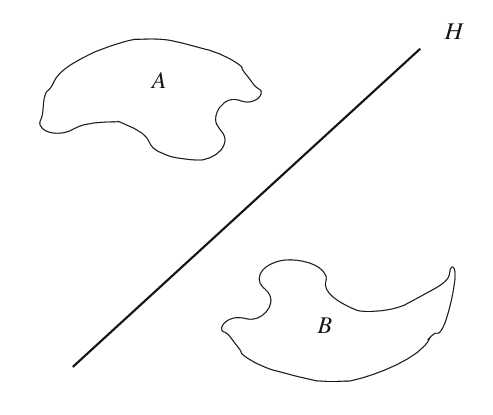
\includegraphics[width=0.5\linewidth]{Images/Seperation by Hyperplanes.png}
    \caption{Seperation by Hyperplanes, from Brezis}
\end{figure}

\begin{lem}
    Let $C\subset E$ be an open convex set with $0\in C,$ then define $p: E\to \bbR$ by
    \[p(x) = \{\alpha > 0 \; | \: \frac{1}{\alpha}x \in C\}.\] Then $p$ is a seminorm such that there is some $M\in \bbR$ with $0\leq p(x) \leq M\|x\|$ for any $x\in E,$ and 
    \[C = \{x\in E \: | \; p(x) < 1\}.\]
\end{lem}
In a way, we can think of $\alpha$ as the smallest number required to pull an element into $C$ when dividing it by $\alpha.$ 
\begin{proof}
    We have positive definitiveness by definition. By the openness of $C \ni 0,$ we get that there exists some $r>0$ such that $B_r(0) \subset C.$ Informally, we can think of it taking more of an effort to pull in an $x$ into $B_r(0)$ than it is to pull it into $C$ (since $C$ is `larger'). Let $\alpha = \frac{\|x\|}{r},$ then we get that if $x\in E,$ 
    \[\frac{1}{\alpha}x = \frac{x}{\|x\|}r \in B_r(0) \implies \frac{1}{\alpha}\in C,\] and thus $p(x)\leq \frac{\|x\|}{r}$ by definition. 

    Let $x\in C,$ then for small $\epsilon>0,$ we have by the openness of $C$ (and convexity) that $(1  +\epsilon)x \in C,$ and thus 
    \[p(x)\leq \frac{1}{1+\epsilon}< 1.\] Thus, $C \subset \{x\in E \: | \; p(x) < 1\}.$ Let $x\in E$ with $p(x)< 1,$ then there is an $\alpha$ such that
    \[\frac{1}{\alpha}x \in C \implies \alpha(\frac{1}{\alpha} x) + (1-\alpha)(0) = x\in C.\] To prove the triangle inequality, we note that if $x,y\in E,$ $p(x), p(y) >1,$ and thus there exists an $\epsilon>0$ such that 
    \[\frac{x}{p(x) + \epsilon}\in C, \qquad \frac{y}{p(y) + \epsilon} \in C \implies \frac{x}{p(x)+ \epsilon}< 1 \implies x < p(x) + \epsilon.\] Letting $ 0 \leq t = \frac{p(x) + \epsilon}{p(x) + p(y) + 2\epsilon}\leq 1,$ we see that using the convexity of $C$ that 
    \[\frac{x + y}{p(x) + p(y) + 2\epsilon}\in C\] and thus we have that if we set $\alpha = p(x) + p(y) + 2\epsilon,$ then we see that 
    \[p(x + y) \leq \alpha = p(x) + p(y) + 2\epsilon.\] 
\end{proof}

\begin{lem}
    Let $C\subset E$ be a  nonempty open convex set and suppose $x_0 \in E\sm C.$ Then there exists an $f\in \mathcal{L}(E, \bbR)$ such that $f(x) < f(x_0)$ for all $x \in C.$ 
\end{lem}

\begin{proof}
    After translating (linear functions don't give a shit about translating) such that $0\in C,$ we let $G = \bbR x_0$ be the linear subspace of the line of $x_0,$ and we define the functional
    \[g: G \to \bbR \quad g(t x_0) = t.\] Consider the \textbf{gauge} defined in Lemma 2, then we claim that $g(x) \leq p(x):$ Obviously, $g(x_0) = 1,$ and thus
    \[g(x_0)\leq p(x_0) \implies g(tx_0) \leq p(t x_0) \implies g(x) \leq p(x)\] From the Hahn-Banach Theorem (Thm 16), we get that there exists an extension of $f: E\to \bbR$ such that $f(x)\leq p(x) \leq M\|x\|, \qquad \forall x\in E,$ where the $M$ comes from Lemma 2 above. Thus, we get that $f\in \mathcal{L}(E, \bbR)$ and
    \[f(x_0) = 1 \implies f(x) \leq p(x) < 1 = f(x_0) \; \forall x\in C.\]
\end{proof}

\begin{thm}
    (Geometric Hahn-Banach, first form) Suppose $A, B \subset E$ be nonempty, convex, and disjoint. Suppose that $A$ is open. Then there exists a closed hyperplane that separates $A$ and $B.$ 
\end{thm}
\begin{proof}
    Let $C = A -  B.$ Then $C$ is convex. Since $C = \bigcup_{y\in B}(A - y),$ then $C$ is open, and $0 \notin C.$ By Lemma 3 there is some $f\in \mathcal{L}(E, \bbR)$ such that $f(z) < f(0) = 0$ for all $z\in C.$ Thus, we have that if $x \in A$ and $y \in B,$ then 
    \[f(z) = f(x - y) = f(x) - f(y) < 0 \implies f(x) - f(y) \implies \sup_{x\in A}f(x)\leq \alpha \leq \sup_{y\in B}f(y).\]
\end{proof}



\begin{thm}
    (Geometric Hahn-Banach, second form) Suppose $A, B \subset E$ be nonempty, convex, and disjoint. Suppose that $A$ is closed and $B$ is compact, then there exists a closed hyperplane that strictly separates $A$ and $B.$
\end{thm}
\begin{proof}
    Again, we make $C = A - B,$ then $C$ is convex, $0\notin C,$ and $C$ is closed (easy to see with the compactness of $B$). By the the Geometric first form of the Hahn Banach Theorem (Thm 17), we get that a closed hyperplane $H = [f = \alpha]$ that separates $C$ and $B_r(0).$ Thus, we get that for all $x\in A,$ $y\in B,$ and $z\in B_1(0),$ we get
    \[f(x - y) \leq f(rz) \leq \pm r \|f\|.\] Let $\epsilon = \frac{r}{2}\|f\| >0,$ we see that 
    \[f(x) + \epsilon \leq f(y) - \epsilon  \implies \sup_{x \in A}f(x) + \epsilon \leq \alpha\leq \inf_{y\in B}f(y) - \epsilon.\]
\end{proof}

We end with the most famous corollary of the Hahn Banach Theorem, an easy way for checking for density.

\begin{cor}
    Let $F\subset E$ be a linear subspace such that $\overline{F} \neq E,$ then there exists some $f\in \mathcal{E, \bbR}$ with $f \not \equiv 0$ such that for all $x\in F,$ we have that 
    \[\langle f, x \rangle = 0.\]
\end{cor}
\begin{proof}
    Let $x_0 \in E$ with $x_0 \in \overline{F}.$ We can apply the second form of the geometric Hahn-Banach Theorem (Thm 18) since $\{x_0\}$ is compact that $\overline{F}$ is closed. Thus, there exists a closed hyperplane $H = [f = \alpha]$ that strictly seperates the two, that is, for any $x\in \overline{F},$
    \[\langle f, x \rangle < \alpha < \langle f , x_0\rangle \implies \langle f, x\rangle = \equiv 0\] since $\lambda \langle f , x \rangle  < \alpha$ for every $\lambda \in \bbR.$
\end{proof}
\newpage
\subsection{Bonus Problem Session: Riesz Representation Theorem}
\begin{defn}
    The \textbf{variation} of a function $\alpha: [a,b]\to \bbR$ is defined as 
    \[V_a^x(\alpha) = \sup_{P} \sum |\Delta \alpha_i|,\] where $P$ is a partition on $[a,x].$
\end{defn}
\begin{defn}
    The \textbf{total variation} of $\alpha$ $V_a^b(\alpha).$
\end{defn}
\begin{defn}
    We say $\alpha$ has bounded variation if 
    \[V_a^b(\alpha) < \infty.\] We denote the space of all functions with bounded variation as $BV.$
\end{defn}
\begin{thm}
(Jordan Decomposition Theorem)
    If $\alpha \in BV([a,b]),$ then there exist $\alpha^+$ and $\alpha^-$ such that 
    \[\alpha = \alpha^+ - \alpha^-\] and 
    \[V_a^b(\alpha) = V_a^b(\alpha^+) + V_a^b(\alpha^-).\] 
\end{thm}
For the proof of this, define 
\[\alpha^+(0) := \alpha(a), \qquad \alpha^+(x) = \sup_P \sum_P \max\{0, \Delta \alpha_i\} + \alpha(a)\]
\[\alpha^-(0) := \alpha(a), \qquad \alpha^-(x) = \sup_P \sum_P \max\{0, -\Delta \alpha_i\}\]

(A version of the Riesz Representation Theorem)
\begin{prop}
    For all $F\in (C([a,b]))^*,$ there exists an $\alpha \in BV([a,b])$ such that for all $f\in C([a,b]),$ 
    \[F(f) = \int_a^b fd\alpha.\]
\end{prop}
\begin{pf}
    Obviously, $F(f)$ is a linear functional. To show that it is bounded, consider that for any $f\in C([a,b])$ with $\|f\| \leq 1,$ we have that 
    \[\|F(f)\| \leq \int_a^b f d\alpha = \int_a^bf d\alpha^+ - \int_a^b fd\alpha^- \leq \alpha^+(b) - \alpha^+(a) - \alpha^-(b) + \alpha^-(a) < \infty.\]

    We let $F \in C([a,b])^*.$ Since $C([a,b]) \subset C^b([a,b]),$ then by the Hahn Banach Theorem (Thm 16), there exists some linear functional $G \in (C^b([a,b]))^*$ such that $G|_{C([a,b])} = F$ and $\|G\| = \|F\|.$ Define
    \[\alpha(a):= 0, \qquad \alpha(x) := G(\chi_{[a,x]}).\] Then note that 
    \[\alpha(y)- \alpha(x) = G(\chi_{[a,y]}) - G(\chi_{[a,x]}) = G(\chi_{[a,y]} - G(\chi_{[a,x]})) = G(\chi_{[x,y]}).\] To see that $\alpha$ has bounded variation, let $P$ be a partition of $[a,b].$ Then we have that 
    \[\sum_P |\Delta \alpha_i| = \sum_P \text{sign}(\Delta \alpha_i) \Delta \alpha_i = \sum_P \text{sign}(\Delta \alpha_i) G(\chi_{[x_{i-1}, x_i]}) = G(\sum_P\text{sign}(\Delta \alpha_i) \chi(_{[x_{i-1}, x_i]})) \leq \|G\| < \infty.\] 

    Let $f\in C([a,b])$ and choose $\delta>0$ such that $|f(x) - f(y)|< \frac{\epsilon}{2\|F\|}$ from uniform continuity. Choose $P$ fine such that 
    \[\Bigg|\sum_P f(x_i) \Delta \alpha_i - \int_a^b f d\alpha \Bigg|< \frac{\epsilon}{2}.\] Define
    \[g:= \sum_P f(x_i) \chi_{[x_{i-1}, x_i]}.\] Then 
    \begin{align*}
        \left| F(f)- \int_a^b f d\alpha\right| &\leq \left|F(f) - G(g)\right| + \left|G(g) + \int_a^b fd\alpha\right|\\
        &< |F(f) - F(g)| + \frac{\epsilon}{2}\\
        &= |F(f - g)| + \frac{\epsilon}{2}\\
        &\leq \|F\|\|f - g\|\frac{\epsilon}{2\|F\|} + \frac{\epsilon}{2}\\
        &< \|F\|\frac{\epsilon}{2\|F\|} + \frac{\epsilon}{2}\\
        &= \epsilon.
    \end{align*}
\end{pf}



\newpage
\subsection{Wednesday, Jan 29: Midterm}
We had a midterm! I'll post the questions and my answers later. The first question was so ass though. It was not a hard midterm, but it felt like Soug was testing how fast we could write. Here are the questions:

\begin{enumerate}
    \item \begin{problem}
    Define three functions, $\beta_1, \beta_2, \beta_3$ as follows: $\beta_j(x) = 0$ if $x<0,$ $\beta_j = 1$ if $x>0$ for $j = 1,2,3;$ and $\beta_1(0) = 0,$ $\beta_2(0) = 1,$ and $\beta_3(0) = \frac{1}{2}.$ Let $f$ be a bounded function on $[-1,1].$ 
\end{problem}
\begin{enumerate}
    \item 
    \begin{problem}
        Prove that $f\in \mathcal{R}(\beta_1)$ if and only if $f(0 + ) = f(0)$ and that then $\int f d\beta_1 = f(0).$
    \end{problem}
    \item 
    \begin{problem}
        State and prove a similar result for $\beta_2.$
    \end{problem}
    \item 
    \begin{problem}
            Prove that $f\in \mathcal{R}(\beta_3)$ if and only if $f$ is continuous at $0.$
    \end{problem}
    \item 
    \begin{problem}
        If $f$ is continuous at $0,$ prove that 
        \[\int f d\beta_1 = \int f d\beta_2 = \int f d\beta_3 = f(0).\] 
    \end{problem}
\end{enumerate}
\item Determine the Fourier coefficients:
\[\hat{f}(n) = \frac{1}{2\pi}\int_{-\pi}^\pi f(x)e^{-inx}dx,\] where 
\[f(x) = \begin{cases}
    -1, \qquad \: x\in [-\pi, 0],\\
    1, \qquad \;\;\:x\in(0,\pi]
\end{cases}\]
and then use them to compute
\[\sum_{k=0}^\infty \frac{1}{(2k + 1)^2}\]
\item A map $\phi: V \to V$ where $V$ is a vector space over $\bbR$ is \textbf{affine} if there exists some $x_0 \in V$ and a linear map $T: V \to V$ such that for all $x\in V$ we have $\phi(x) = x_0 + T(x).$ Prove that $\phi: V\to V$ is affine if and only if $\phi(\sum \lambda_i x_i) = \sum \lambda_i \phi(x_i)$ for all $\lambda_i$ such that $\sum_{i=1}^n \lambda_i = 1.$
\item Show that $C^n([0,1])$ is a Banach space with the norm 
\[\|f\| = \sup_n \sup_{x\in [0,1]}|f^n(x)|\]
\item Show that the normed space $\cal L$ of all real value Lipshitz function on $\bbR$ that are equal to $0$ at the origin under the norm
\[\|f\| = \sup_{x,y \in \bbR}\frac{|f(x) - f(y)|}{|x-y|}\] is Banach.
\end{enumerate}

\newpage
\subsection{Friday, Jan 31: The Baire, Uniform Boundedness, and Open Mapping Theorems}
Big day today.
\begin{thm} (Baire's Category Theorem)
    Suppose $X$ is a complete metric space and we can write it as \[X = \bigcup_{i=1}^\infty F_i,\] where each $F_i$ is closed. Then there exists some $i$ such that $\text{int}(F_i) \neq \emptyset.$
\end{thm}
\begin{proof}
    We will first prove that if $G_n$ is a sequence such that each $G_n$ is open and dense, then $\bigcap G_n$ is dense in $X.$ To do this, we let $x\in X$ and $\epsilon>0.$ Consider that since $G_1$ is dense in $X,$ then there exists some $x_1 \in G_1\cap B_\epsilon(x).$ Since $G_1 \cap B_\epsilon(x)$ is open, then there exists some $r>0$ such that 
    \[\overline{B_{\frac{r_1}{2}}(x_1)}\subset G_1 \cap B_\epsilon(x)\] Since $G_2$ is dense in $X,$ there exists some \[x_2 \in G_2 \cap B_{\frac{r_1}{2}}(x_1)\subset G_1 \cap B_\epsilon(x),\] and so there exists some $r_2 >0$ such that 
    \[\overline{B_{\frac{r_2}{2}}}(x_2)\subset G_2 \cap B_\frac{r_1}{2}(x_1)\]
    
    Thus, we create the sequence $x_n$ such that \[x_n \in G_n \cap B_\frac{r_{n-1}}{2}(x_{n-1}).\] Evidently, $(x_n)$ is Cauchy since $r_n \to 0$ and thus by the completeness of $X,$ $x_n \to x_\infty \in G_n$ for all $G_n.$ Thus, \[x_\infty \in \bigcap G_n \cap B_\epsilon(x),\] and so $\bigcap G_n$ is dense in $X.$

    With this now proven, we note that if $F$ is closed with an empty interior, then $F^c$ is open and dense. Thus, suppose the interior of all $F_n$ is empty, then 
    \[\emptyset = X^c = \left(\bigcup F_n\right)^c = \bigcap F_n^c,\] and thus the emptyset is dense in $X,$ which is obviously false (unless $X$ is the emptyset). 
\end{proof}
Now for the Uniform Boundedness, which states that under certain conditions, pointwise convergence implies uniform convergence.
\begin{thm}
    (Banach-Steinhaus) Uniform Boundedness Theorem. Let $E,$ $F$ be Banach, and suppose $(T_\alpha)_{\alpha \in \mathcal{A}} \in \mathcal{L}(E, F).$ Suppose 
    \[\sup_{\alpha \in \mathcal{A}}\|T_\alpha x\| < \infty \qquad \forall  \; x\in E,\] then there exists some $c$ such that 
    \begin{align}
        \sup_{\alpha\in \mathcal{A}}\|T_\alpha x \| < c\|x\| \qquad \forall \; x\in E.
    \end{align}
    That is, 
    \[\sup_{\alpha\in \mathcal{A}}\|T_\alpha\|_{\mathcal{L}(E, F)} <\infty\]
\end{thm}
\begin{proof}
    Define
    \[C_n := \{x \in E \; ; \; \|T_\alpha x\| \leq n\}.\] We know that $C_n \subset C_{n+1}$ and by assumption that $\bigcup C_n = E.$ Closedeness is obvious. From Theorem 19 (Baire's), we have that there exists some $C_n$ with nonempty interior. That is, there is some $x_0\in C_{n_0}$ with $r>0$ such that $B_r(x_0)\subset C_{n_0}.$ Thus, for all $x\in B_r(x_0),$
    \[\|T_{n_0}(x)\| \leq n_0 \implies \|T_{n_0}(x_0 + rz)\| \leq n_0, \qquad \|z\| \leq 1,\] thus, by linearity of the $T,$ we find that 
    \[T_{n_0}(z) \leq \frac{n_0 + \|T_{n_0}x_0\|}{r},\] implying uniform boundedness.
\end{proof}

We provide a couple of corollaries:
\begin{cor}
    Suppose $E, F$ are Banach and $(T_n)\in \mathcal{L}(E, F)$ such that $\lim_{n\to \infty} T_n(x) = T(x),$ then 
    \begin{enumerate}
    \item \[\sup_{n} \|T_n\| < \infty\]
        \item \[T\in \mathcal{L}(E, F)\]
        \item \[\|T\| \leq \liminf_{n\to \infty}\|T_n\|\]
    \end{enumerate}
\end{cor}
\begin{proof}
    By the existence of the limit, we have that the $(T_n)$ are pointwise bounded, and thus (1) follows from Theorem 20. By taking the limit, we see that if 
    \[\|T_nx\| \leq c\|x\| \implies \|Tx\| \leq c\|x\|,\] and so $T\in \mathcal{L}(E,F).$ If we let $x\in E,$ then we have that 
    \[\|T_nx|\|\leq \|T_n\|\|x\|,\] and so (3) is proved.
\end{proof}

\begin{cor}
    Suppose $E$ is Banach and $A\subset E.$ If $f(A)$ is bounded for any $f\in E^*$, then $A$ is bounded.  
\end{cor}
\begin{proof}
    From Theorem 20, we let $E ``="E^*,$ $F``=" \bbR,$ and $\mathcal{A} ``=" A.$ Then for all $a\in A,$ 
    \[T_a(f) := f(a), \qquad f\in E^*.\] By the boundedness of $f(A),$ we have that 
    \[\sup_{a\in A}\|T_a f\|< \infty \qquad \forall \; a\in A,\] and so by Theorem 20:
    \[|f(b)| \leq c\|f\| \qquad \forall \; b\in B,\quad f\in E^*,\] and so 
    \[|b| \leq c \qquad \forall \; b\in B\]
\end{proof}
I don't really fuck with Theorem 20. I do fuck with the open mapping theorem, although it's proof is rough.
\begin{thm}
(Open Mapping Theorem)
    Suppose $E,$ $F$ are Banach and $T\in \mathcal{E, F}$ such that $T$ is surjective. Then there exists some $c>0$ such that 
    \begin{align}
        B^F_c(0)\subset T(B_1^E(0))
    \end{align}
\end{thm}
\begin{proof}
    We claim that (9) implies that $T$ is open. Indeed, let $U$ be open in $E,$ then if $y_0 \in T(U)$ (and let's say $y_0 = Tx_0,$ where $x_0 \in U$), then by the openness of $U,$ there exists some $r>0$ such that $B_r^E(x_0)\subset U.$ Thus, 
    \[B_r^E(x_0) = x_0 + B_r^E(0)\subset U,\] and so
    \begin{align}
    y_0 + T(B_r^E(0))\subset T(U).    
    \end{align}
    By (9), we have that there exists some $c>0$ such that 
    \[B_c^F(0)\subset T(B_1^E(0)) \implies B_{rc}^F(0)\subset T(B_r^E(0))\] So by (10), we know that
    \[T(B_{rc}(y_0))\subset T(U),\] and so $T(U)$ is open.

    \begin{enumerate}
        \item Our first step is to show that if $T$ is a linear surjective map from $E$ to $F,$ then there exists some $c>0$ such that 
        \[B_{2c}^E(0)\subset \overline{B^F_1(0)}.\]

        To show this, we let 
        \[X_n = n\overline{T(B^F_1(0))}.\] Obviously, $X_n$ is closed, and since $T$ is bounded, we have that $T(E) = F$ is bounded, and thus
        \[F = \bigcup X_n.\] Since $F$ is complete, we use Baire's Category Theorem (Theorem 19) to say that there exists some $i$ such that $\text{int}X_n \neq \emptyset.$ That is, there is some $y_0 \in X_n$ and $c>0$ such that 
        \[B_{4c}(y_0)\subset \overline{T(B^F_1(0))}\] and by symmetry
        \[B_{4c}(-y_0)\subset \overline{T(B_1^F(0))}.\]
        Thus, we get that by adding them up:
        \[B^E_{4c}(0) \subset 2\overline{T(B_1^F(0))} \implies B^E_{2c}(0) \subset \overline{T(B_1^F(0))}.\]

        \item The second step is that if $T$ is a linear continuous from $E$ to $F,$ then step (a) implies that 
        \[B_c^F(0)\subset T(B_1^E(0)).\]

        To show this, let $y_0 \in B_c^F(0),$ that is $\|y_0\|  < c.$ We need to find an $x_0\in E$ with $\|x_0\| < 1$ such that $Tx_0 = y_0.$ Let $\epsilon>0.$ By (a), we know that there exists some $z\in E$ with $\|z_1\|< \frac{1}{2}$ such that 
        \[\|y - Tz_1\|< \epsilon.\] Fixing $\epsilon = \frac{c}{2},$ we have that 
        \[\|y - Tz_1\|< \frac{c}{2}.\] Thus, there exists some $\|z_2\| < \frac{1}{4}$ such that 
        \[\|(y - Tz_1) - Tz_2\|< \frac{c}{4},\] and so on. Thus, we have that  for $\|z_n\|< \frac{1}{2^n},$
        \[\|y - T(z_1 + z_2 + \dots + z_n)\|< \frac{e}{2^n},\] and so the sequence 
        \[x_n = \sum_{i=1}^n z_i\] is Cauchy, and thus converges to some $x_0$ by the completeness of $E.$ We have $\|x_0\|< 1$ and $y= Tx.$
    \end{enumerate}
\end{proof}

\begin{cor}
    Suppose $E,$ $F$ are Banach and $T\in \mathcal{E, F}$ such that $T$ is bijective. Then $T^{-1}\in \mathcal{L}(F, E).$
\end{cor}
\begin{cor}
    Let $E$ be a Banach space for two norms $\|\cdot\|_1$ and $\|\cdot\|_2.$ If there exists a constant $C>0$ such that 
    \[\|x\|_2 \leq C\|x\|_1, \qquad \forall\; x\in E,\] then there exists a constant $c>0$ such that 
    \[\|x\|_1 \leq c\|x\|_2, \qquad \forall\; x\in E.\]
\end{cor}
\begin{proof}
    To show the norms are equivalent, consider 
    \[I : (E, \|\cdot\|_1) \to (E, \|\cdot\|_2).\] We know that $I\in \mathcal{L}(E)$ and that $I$ is bijective. By the previous corollary, $I^{-1}\in \mathcal{E},$ and so we are done.
\end{proof}

\begin{thm}
    (Close Graph Theorem) Suppose $E,$ $F$ are Banach and $T: E\to F$ is linear. Then the graph of $T,$ $(G(T))= \{(x, Tx) \; x\in E\},$ is closed in $E\times F$ if and only if $T$ is continuous.
\end{thm}
\begin{proof}
    The backwards direction is obvious. Consider the graph norm
    \[\|\cdot\|_G = \|\cdot\|_E + \|T\cdot\|_F,\] then one can probably see that $E$ is Banach under both norms and obviously,
    \[\|\cdot\|_E \leq \|\cdot\|_G,\] and so by the previous corollary, the norms are equivalent and so there exists some $c>0$ such that 
    \[\|Tx\|_F \leq c\|x\|_E\]
\end{proof}

\newpage
\subsection{Monday, Feb 3: The Weakest Topology}
We spent about 15 minutes today discussing how badly we did on the midterm. If only question 1 wasn't god awful huh. Anyways he talked about how his grading scheme is:
\[10\% \;\; \text{HW} \qquad 40\%\;\; \text{Midterm} \qquad 50\% \; \text{Final}\]
Discuss among yourselves how stupid $10\%$ homework is when we had a 27 problem PSET (mostly Brezis problems) due on Week 6. But he assured us if we got a 30 on the midterm and did well on the final we would get an A. So I am not worried.

Then we proved the Open Mapping Theorem (which is proven above, where I stated it) and introduced weak convergence.

\begin{rem}
    We construct the weak topology from $X,$ a set, to $(Y_i)_{i\in I},$ a collection of topological spaces, such that it makes every map continuous. Let 
    \[\varphi_i: X \to Y_i\] be continuous. Let $\omega_i \subset Y_i$ be open, then $(U_\lambda)_{\lambda \in |\Lambda} = \varphi^{-1}(\omega_i)$ is a collection of open sets in $X.$ Consider $\bigcap_{\lambda \in \Gamma}U_\lambda,$ where $\Gamma \subset \Lambda$ is finite. Then the finite intersection is open, and call this collection of intersections $\Phi.$ Call $\mathcal{F}$ the family of arbitrary unions of $\Phi.$ We say $X$ is equipped with $\mathcal{F},$ which is the weakest topology associated with the $\varphi_i.$
\end{rem}

\begin{prop}
    Suppose $(x_n)\in X$ with $x_n \to x.$ Then for all $i \in I,$ we have that $\varphi_i(x_n) \to \varphi(x).$ 
\end{prop}

\begin{prop}
    Suppose $Z$ is a topological space and $\psi: Z \to X.$ Then $\psi$ is continuous if and only if 
    \[\varphi_i \circ \psi: Z \to X\] is continuous for all $i\in I.$
\end{prop}


\newpage
\subsection{Wednesday, Feb 5: Weak Convergence}
From now on, whenever you see a $\varphi_f(x),$ think of it as $\langle f, x\rangle$
\begin{defn}
    The \textbf{weak topology} of $E,$ $\sigma(E, E^*)$ is the coarsest topology of $E$ associated with the collection $(\varphi_f)_{f\in E^*}$
\end{defn}
\begin{prop}
    Suppose $x_0 \in E,$ then given $\epsilon>0$ and a finite set $\{f_i\}_{i\in [k]},$ define
    \[V:= \{x \in E \; ; \; |\langle f_i, x-x_0\rangle| < \epsilon, \quad \forall \; i \in [k]\}.\] By varying the variables involved, we obtain a basis of the neighborhoods of $x_0.$
\end{prop}
\begin{proof}
    We have that 
    \[V = \bigcap_{i\in [k]}\varphi_{f_i}^{-1}(\langle f, x_0 \rangle - \epsilon, \langle f, x_0 \rangle + \epsilon),\] and thus $V$ is open in $\sigma(E, E*).$ To see that an open neighborhood contains $V,$ see the construction of the topology.
\end{proof}
\begin{thm}
    Suppose $(x_n) \in E,$ then:
    \begin{enumerate}
        \item $x_n\rightharpoonup x$  if and only if $\langle f, x_n\rangle \to \langle f, x\rangle$ for all $f\in E^*.$
        \item If $x_n \to x,$ then $x_n \rightharpoonup x.$
        \item If $x_n \rightharpoonup x,$ then $\|x_n\|$ is bounded and $\|x\|\leq \liminf \|x_n\|.$
        \item If $x_n \rightharpoonup x$ and $f_n \to f$ in $E^*,$ then $\langle f_n, x_n \rangle \to \langle f, x\rangle.$
    \end{enumerate}
\end{thm}
\begin{proof}
    We prove these one by one:
    \begin{enumerate}
        \item Suppose $x_n \rightharpoonup x,$ then since $f\in E^*$ then $f$ is continuous and thus $f(x_n) \to f(x).$ See proposition 7.
        \item By (a), we have that it suffices to show $\langle f, x_n\rangle \to \langle f, x\rangle.$ Let $f\in E^*,$ then 
        \[\|\langle f, x_n \rangle - \langle f, x\rangle\|\leq \|f\|\|x - x_n\| < \epsilon.\]
        \item By the uniform boundedness principle, we have that 
        \[\|\langle f, x_n\rangle\| \leq \|f\|\|x_n\| \implies |\langle f, x\rangle\| \leq \liminf \|f\|\|x_n\| \implies \|x\|\leq \liminf \|x_n\|.\]
        \item 
        \[\|\langle f_n, x_n \rangle- \langle f, x\rangle\| \leq \|\langle f_n - f, x_n \rangle\| + \|\langle f, x_n - x\rangle\|,\] which is enough by (a) and (c).
    \end{enumerate}
\end{proof}
\begin{prop}
    If $\dim E < \infty,$ then $x_n \rightharpoonup x$ if and only if $x_n \to x.$
\end{prop}
\begin{proof}
    One direction is clear. Let $U$ be strongly open around some $x_0 \in E.$ We need to find some $V\subset U$ such that $x_0 \in V$ and $V$ is open in $\sigma(E, E^*).$ Thus, it suffices to find $\{f_1, f_2, \dots\} \subset E^*$ such that for all $\epsilon>0,$
    \[V= \{x \in E \; ; \; |\langle f_i, x-x_0\rangle| < \epsilon\}.\] Let $r>0$ such that $B_r(x_0)\subset U.$ Since $E$ is finite, pick a basis $e_1, e_2, \dots, e_k$ such that $x = \sum_{n=1}^k e_nx_n.$ Let $\pi_i: x\to x_i$ be the projection mapping, which is continuous, and thus 
    \[\|x - x_0\|\leq \sum \|\langle \pi_i, x-x_0\rangle\| < \epsilon k\] for all $x\in V.$ Choose $\epsilon = \frac{r}{k}$ and we are done.
\end{proof}

We provide now an example of why the above proposition does not hold for infinite dimensions, that is, there exists open and closed sets in the strong topology that are \textit{never} open or closed in the weak topology.
\begin{exmp}
    We will show that the unit sphere, $S,$ which is strongly closed and $U = \{x \in E \; ; \; \|x\| <1\},$ which is strongly open, are not weakly closed and not weakly open (respectively). We will see that
    \[\overline{S}^{\sigma(E, E^*)} = B_E,\] which is the closed unit ball in $E.$ 

    Let $x_0\in E$ with $\|x_0\| \leq 1.$ Let $x_0\in V$ be a neighborhood, it suffices to see that $V \cap S \neq \emptyset$ for every $V$ in order for $x_0\in \overline{S}^{\sigma(E, E^*)}.$ We know by proposition 9 that there exists some $\{f_1, f_2, \dots, f_k\}\subset E^*$ such that 
    \[V = \{x \in E \; ; \; |\langle f, x-x_0\rangle| < \epsilon\}.\] There exists some $y_0 \neq 0$ such that for every $i \in [k],$ we have that $\langle f_i, y_0\rangle = 0.$ This $y_0$ exists, since otherwise $\dim E < \infty$\footnote{Prove this more later.} Define $g(t) = \|x_0 + ty_0\|,$ then $g(0) < 1$ and $g(t) \to \infty$ as $t\to \infty,$ so there must exist some $t_0$ such that $g(t_0) = 1.$ Thus, we have that $g(t_0) = x_0 + t_0y_0 \in V \cap S.$

    For the other inclusion, we have that $S\subset B_E,$ and so $\overline{S}^{\sigma(E, E^*)}\subset \overline{B_E}^{\sigma(E, E^*)},$ so it suffices to show that $B_E$ is weakly closed, but this comes from the fact that 
    \[B_E = \bigcap_{\substack{f\in E^*\\\|f\| \leq 1}} \{x \in E \; ; \; |\langle f, x\rangle| \leq 1\}\]

    Thus, we see that $S$ is not weakly closed. To see that $U$ is not weakly open, suppose it is, then $U^c$ is weakly closed, but then 
    \[S = B_E \cap U^c\] is weakly closed, which is a contradiction.
\end{exmp}

\subsection{Friday, Feb 7: Weak Convexity}
We mostly talked about example $3$ above, but also stated a few results. Recall that in infinite dimensions, strongly closed sets are not necessarily weakly closed. 
\begin{thm}
    Suppose $C\subset E$ is convex. Then $C$ is strongly closed if and only if $C$ is weakly closed.
\end{thm}
\begin{proof}
    If $C$ is weakly closed, then of course it is strongly closed. 

    Suppose $C$ is strongly closed, then let $x_0 \in E\setminus C.$ $\{x_0\}$ is closed (strongly), convex, and nonempty. $C$ is nonempty, closed, and convex, and thus we apply Hahn-Banach to find a continuous functional $f: E \to \bbR.$ such that 
    \[f(x_0) < f(\alpha) < f(C).\] Consider that 
    \[V:= \{x\in E \; : \; \langle f, x \rangle < \alpha\}\] is an open neighborhood containing $x_0.$ Thus, $x_0 \in V \subset C^c$ and so $C^c$ is weakly open and thus $C$ is weakly closed.
\end{proof}
\begin{defn}
    We say that $f$ is \textbf{left semi continuous} at$x_0$ if \[f(x_0) \leq \liminf{x\to x_0} f(x)\]
\end{defn}
\begin{cor}
    Suppose $\varphi: (-\infty, \infty]$ is convex and l.s.c. in the strong topoology, then $\varphi$ is l.s.c in the weak topology.
\end{cor}
\begin{cor}
    (Mazur) Suppose $x_n \rightharpoonup x.$ Then there exists $(y_n)\to x$ such that $y_n \in \text{Conv}[(x_n)].$
\end{cor}

\newpage
\subsection{Monday, Feb 10: Adjoint Operators}
For this entire lecture, we suppose $E,F$ are Banach, and $A: D(A)\subset E \to F$ is an unbounded linear operator.
\begin{defn}
We say that $A$ is \textbf{densely defined} if $\overline{D(A)} = E.$
\end{defn}
\begin{defn}
    We say that $A$ is bounded if $D(A) = E$ and there exists some $c>0$ such that for all $u \in E,$ we have that $\|A(u)\|_F \leq c\|u\|_E.$
\end{defn}
\begin{defn}
    Suppose $A: D(A)\subset E \to F$ is a densely defined unbounded linear operator. We define the \textbf{adjoint} $A^*: D(A^*)\subset F^* \to E^*$ such that 
    \[D(A^*) := \{v\in F^* \; : \exists c>0 \text{ st}\; \langle v, Au\rangle \leq c \|u\|_E\} \; \forall u \in D(A)\}\]
    \[\langle v, Au\rangle = \langle A^*v , u\rangle \qquad \forall\:v\in D(A^*), \; \forall \:u\in D(A).\]
\end{defn}
We remark that $D(A^*)$ is a linear subspace and live the proof for you.
\begin{rem}
    To prove the existence of such an operator, we use H-B. Define $g: D(A)\to \bbR$ such that $g_v(u) = \langle v, Au\rangle,$ then extend $g$ to $E$ using Hahn-Banach to some $f: E\to \bbR$ such that $|f(u)|\leq c\|u\|_E \implies f\in E^*.$ Define $A^*v = f.$ $A^*$ is unique because $A$ is densely defined..
\end{rem}
\begin{prop}
    If $A$ is bounded, then $A^*$ is bounded. Moreover, 
    \[\|A\|_{{\cal L}(E, F)}= \|A^*\|_{{\cal L}(F^*, E^*)}\]
\end{prop}
\begin{proof}
    We have that 
    \[|\langle A^*v, u\rangle| = |\langle v, A u\rangle|\leq \|v\|\|A\|\|u\|\]
    and thus 
    \[\|A^*v\|\leq \|v\|\|A\| \implies \|A^*\| = \sup_{\|v\|\leq 1} \|A^* v\| \leq \|A\|.\]
    For the other side, we have that 
    \[|\langle v, A u\rangle|\leq \|v\|\|A^*\|\|u\| \implies \|Au\| = \sup_{\|v\| \leq 1}|\langle v, Au| \leq \|A^*\|\|u\|.\] Taking supremums, we see that 
    \[\|A\|\leq \|A^*\|\]
\end{proof}

\begin{prop}
    If $A$ is densely defined unbounded linear operator, then $A^*$ is closed.
\end{prop}
\begin{proof}
    Suppose $(v_n)\in D(A^*)$ such that $v_n \to v$ in $F^*$ and $A^*v_n \to f$ in $E^*,$
 then 
\[\langle f, u\rangle\leftarrow\langle A^*v_n, u\rangle = \langle v_n, Au\rangle \to \langle v, Au \rangle.\] Thus, $v\in D(A^*)$ since $|\langle v, Au\rangle| \leq \|f\|\|u\|$ for any $u\in D(A)$ and $A^*v = f.$
 \end{proof}

 \begin{prop}
     The following statements hold:
     \[N(A) = R(A^*)^\perp\]
     \[N(A^*) = R(A)^\perp\]
     \[N(A)^\perp \supset \overline{R(A^*)}\]
     \[N(A^*)^\perp = \overline{R(A)}\]
 \end{prop}
 We proved this in our homework.
 \begin{rem}
     The inclusion in (3) is an inclusion in reflexive spaces since in the weak topology, $N(A)^\perp = \overline{R(A^*)}^{\sigma(E, E^*)}$
 \end{rem}

 \newpage
 \subsection{Friday, Feb 14: The Weak $\star$ Topology}
\begin{defn}
    The weak $^*$ topology $\sigma(E^*, E)$ is the coarsest topology $E^*$  such that for every $x\in E,$ the linear function $\varphi_x: E^*\to \bbR$ defined by $\varphi_x(f)= \langle f, x\rangle$ is continuous. 
\end{defn}
\begin{rem}
    Since $E\subset E^{**},$ then $\sigma(E^*, E)$ is coarser than $\sigma(E^*, E^{**}).$
\end{rem}
\begin{prop}
    Let $f_0 \in E^*,$ then given ${x_1, \dots, x_k}\in E$ and $\epsilon >0,$ a neighborhood of $f_0$ is 
    \[V:= \{f\in E^* \; : \; |\langle f - f_0, x_i \rangle|< \epsilon, \; \; \forall \;i\in [k]\}\]
\end{prop}

\begin{thm}
\begin{enumerate}
    \item $f_n\stackrel{\ast}{\rightharpoonup} f$ if and only if $\langle f_n, x\rangle \to \langle f, x\rangle$ for all $x\in E.$
    \item If $f_n \to f,$ then $f_n\rightharpoonup f$ then $f_n\stackrel{\ast}{\rightharpoonup} f$
    \itme If $f_n\stackrel{\ast}{\rightharpoonup} f,$ then $\|f_n\|$ is bounded and $\|f\|\leq \lim\inf \|f_n\|$
    \item If $f_n\stackrel{\ast}{\rightharpoonup} f$ and $x_n \to x,$ then $\langle f_n, x_n\rangle \to \langle f, x\rangle$
\end{enumerate}

\begin{thm}
    The closed unit ball 
    \[B_{E^*} = \{f \in E^* \; : \; \|f\|\leq 1\}\] is compact in $\sigma(E^*, E).$
\end{thm}
That's pretty neat! I'm not going to prove it though!
\end{thm}


\newpage
\subsection{Monday, Feb 17: Reflexive Spaces and Hilbert Spaces}
Today we had double class for some fucking reason. Strap in. Bro didn't prove a thing about reflexive spaces, he just stated the important results. 

\begin{defn}
    Let $E$ be a Banach space and suppose $J: E\to E^{**}$ is the canonical injection. The space $E$ is \textbf{reflexive} if $J$ is surjective.
\end{defn}
\begin{thm}
    Let $E$ be a Banach space. Then $E$ is reflexive is and only if $B_E$ is weakly compact in $\sigma(E, E^*)$
\end{thm}
\begin{thm}
    Let $E$ is be a Banach space and $(x_n)$ is a bounded sequence in $E.$ Then $E$ is reflexive if and only if there exists a subsequence $(x_{n_k})$ that weakly converges in $\sigma(E, E^*).$
\end{thm}

\begin{prop}
    Suppose $M\subset E$ is a closed linear subspace of $E$ reflexive Banach. Then $M$ is a reflexive Banach space. 
\end{prop}

\begin{cor}
    A Banach Space $E$ is reflexive if and only if $E^*$ is reflexive.
\end{cor}

\begin{defn}
    A Banach space is \textbf{uniformly convex} if for all $\epsilon>0,$ there exists a $\delta>0$ such that 
    \[x,y \in E, \|x\|, \|y\|\leq 1 \text{ and } \|x-y\| > \epsilon \implies \|\frac{x + y}{2}\| < 1-\delta\]
\end{defn}
\begin{thm}
    Every uniformly convex Banach space is reflexive.
\end{thm}

\begin{defn}
    Suppose $H$ is a vector space. A \textbf{scalar product} is a bilinear map $(\cdot,\cdot): H\times H \to \bbR$ such that if $u, v\in H,$ then:
    \begin{enumerate}
        \item $(u,v) = (v,u)$
        \item $(u,u) \geq 0$
        \item $(u,u) \neq 0$ if and only if $u\neq 0.$
    \end{enumerate}
\end{defn}
\begin{rem}
    Any vector space $H$ with a scalar product induces a norm of the form 
    \[|u| = (u,u)^\frac{1}{2}.\] 
    Recall the Cauchy-Shwarz inequality:
    \[(u,v)\leq |u|||v|\] and the Parallelogram Law:
    \begin{align}
    |\frac{u + v}{2}|^2 + |\frac{u-v}{2}|^2 = \frac{1}{2}(|u|^2 + |v|^2)    
    \end{align}
    
\end{rem}

\begin{defn}
    A \textbf{Hilbert Space} is a vector space $H$ equipped with a scalar  product such that $H$ is complete for the induced norm.
\end{defn}

\begin{prop}
    $H$ is uniformly convex.
\end{prop}
\begin{proof}
    Let $\epsilon>0$ and $u,v \in H$ with $|u|\leq 1,$ $|v|\leq 1,$ $|u-v|>\epsilon,$ then using (11) we see that
    \[|\frac{u + v}{2}|^2 < 1- \frac{\epsilon^2}{4},\] and so $|\frac{u + v}{2}| < 1-\delta,$ where $\delta$ is chosen smartly from above.
\end{proof}

\begin{thm}
    Let $K\subset H$ be a nonempty closed convex set. For every $f\in H,$ there exists a unique element $u\in K$ such that 
    \begin{align}
    |f-u| = \text{dist}(f, K).    
    \end{align}
    This is equivalent to 
    \begin{align}
        (f-u, u-v) \leq 0, \qquad \forall v\in K.
    \end{align}
\end{thm}
\begin{rem}
    The element $u$ is called the \textbf{projection} of $f$ unto $K$ and denoted by 
    \[u = P_Kf\]
\end{rem}
\begin{proof}
    Let $(v_n)\in K$ such that 
    \[d_n = |f- v_n| \to d = \text{dist}(f, K).\] Let $a = f - v_n$ and $b- f - v_m.$ The parallelogram law (11) says that 
    \[|f - \frac{v_n + v_m}{2}|^2 + |\frac{v_n - v_m}{2}|^2 = \frac{1}{2}(d_n^2 + d_m^2)\] and so
    \[|\frac{v_n - v_m}{2}|^2 \leq \frac{1}{2}(d_n^2 + d_m^2) - d^2 \implies |v_n - v_m| \to 0\]
\end{proof}
Proving the equivalence and the uniqueness is just annoying.
\begin{prop}
    Let $K\subset H$ be nonempty closed convex set, then $P_k$ is a contraction.
\end{prop}

\begin{cor}
    Suppose $M\subset H$ is a closed linear subspace. Then if $f\in H,$ $P_Mf$ is the orthagonal projection and $P_M$ is linear. Moreover,
    \[(f - P_Mf, v) = 0, \qquad \forall u\in M.\]
\end{cor}
\begin{defn}
    By definition,
    \[(f - P_Mf, v - P_Mf) \leq0 \qquad \forall v\in M\] and so for all $t\in \bbR,$
    \[(f - P_Mf, tv - P_Mf) \leq 0\]
\end{defn}

This next theorem is actually astounding. Let $f\in H,$ then the map $u \mapsto (f,u)$ is in $H^*$! That's amazing!
\begin{thm}
    (Riesz) Let $\varphi \in H^*.$ There exists a unique $f\in H$ such that 
    \[\langle \varphi, u\rangle = (f, u) \qquad \forall u \in H.\] Moreover, 
    \[\|f\|_{H} = \|\varphi\|_{H^*}\]
\end{thm}
\begin{proof}
    Let $M = \ker \varphi,$ which is a closed subspace of $H.$ If $M = H,$ then $\varphi \equiv  0$ and so we take $f = 0$ and conclude the proof. Take $M \neq H.$ We claim there exists some $g\in H\setminus M$ such that 
    \[|g| = 1, (g,v) = 0 \qquad \forall v\in M.\] Let $g_0 \in H\setminus M.$ Let $g_1 = P_Mg_0$ and 
    \[g = \frac{(g_0 - g_1)}{|g_0 - g_1|} \implies |g| = 1.\] Let $u\in H$ and (since $g \notin \ker \varphi$) define 
    \[v := u - \frac{\langle \varphi, u\rangle}{\langle\varphi, g\rangle}g \implies (g, v) = (g, u-\frac{\langle \varphi, u\rangle}{\langle\varphi, g\rangle}g)\] Notice that $v\in M,$ and by Corollary 10 we have that $(g,v) = 0$ and so  
    \[(g,u) \langle \varphi, g\rangle = \langle \varphi, u\rangle g\]
    \[\langle \varphi, u\rangle = \langle\varphi, g\rangle (g,u) \implies f = \langle \varphi, g\rangle g\]
\end{proof}

\newpage
\subsection{Friday, Feb 21: The Lax-Milgram Theorem and Orthonormal Bases}
\begin{defn}
    A bilinear form $a: H\times H \to \bbR$ is said to be:
    \begin{enumerate}
        \item \textbf{continuous} if there exists some $C>0$ such that 
        \[|a(u,v)| \leq C\|u\|\|v\|, \qquad \forall u, v \in H\]
        \item \textbf{coercive} if there is a constant $\alpha>0$ such  that 
        \[a(v,v) \geq \alpha\|v\|^2, \qquad \forall v\in H.\]
    \end{enumerate}
\end{defn}
\begin{thm} (Lax-Milgram)
    Assume that $a(u,v)$ is a continuous coercive bilinear form on $H.$ Then, given any $\varphi \in H^*,$ there exists a unique element $u \in H$ such that 
    \[a(u,v) = \langle\varphi, v\rangle, \qquad \forall v\in H.\]
\end{thm}
\begin{proof}
By the Riesz Representation theorem, since $v \mapsto a(u,v)$ is a continuous linear function on $H,$ then there exists some $Au \in H$ such that $a(u,v) = (Au, v),$ where $Au: H\to H$ satisfies the same properties as $a,$ namely
\[|Au| \leq C\|u\|, \qquad (Au, u) \geq \alpha|u|^2.\]
    By the Riesz representation theorem, proving the Lax-Milgram theorem is equivalent to showing that for any $f\in H,$ there exists a unique $u\in H$ such that $Au = f.$ To do this, we need to show that $A$ is injective and surjective.

    We have injective by the fact that $|Au| \leq C\|u\|.$

    We have surjective because $R(A)$ is closed and $R(A)$ is dense. It is closed by coerciveness.
\end{proof}

\begin{defn}
    Let $(E_n)$ be a sequence of closed subspaces of $H$, then $H$ is the \textbf{Hilbert Sum} of the $E_n's$ $H = \oplus_{n} E_n$ if 
    \begin{enumerate}
        \item $E_n$ are mutually orthagonal.
        \item $H = \overline{\text{span}\bigcup_{n=1}^\infty E_n}$
    \end{enumerate}
\end{defn}
Recall Theorem 11 and 12.
\begin{lem}
    Suppose that $(v_n)$ is a sequence in $H$ such that 
    \begin{align}
        (v_m, v_n) = 0, \qquad m\neq n
    \end{align}
    \begin{align}
        \sum_{k=1}^\infty |v_k|^2 < \infty.
    \end{align}
    If $S_n = \sum_{k=1}^n v_n,$ then $S = \lim_{n \to \infty}S_n$ exists and 
    \[|S|^2 = \sum_{k=1}^\infty |v_k|^2\]
\end{lem}
\begin{proof}
    Let $m>n,$ then by the orthogonality of the $(v_n)'$s:
    \[|S_m - S_n|^2 = |\sum_{k= n+1}^m v_k|^2 = \sum_{k=n+1}^m|v_k|^2.\] Since the RHS is the tail of a series that converges, then $|S_m - S_n|^2$ is Cauchy, and since $H$ is complete in its norm, $S = \lim_{n\to \infty} S_n$ exists. It is clear that as $n\to \infty,$ 
    \[|S|^2 = \sum_{k=1}^\infty |v_k|^2\]
\end{proof}

\begin{thm}
    Suppose $H$ is the Hilbert sum of the $E_n'$s. Let $u\in H$ and suppose 
    \[u_n = P_{E_n}u, \qquad S_n = \sum_{k=1}^n u_k\] Then 
    \[\lim_{n\to \infty} S_n = u\] and 
    \begin{align}
        \sum_{k=1}^\infty |u_k|^2 = |u|^2
    \end{align}
\end{thm}
\begin{proof}
    Let $m\neq n,$ then 
    \[(u_n, u_m) = (P_{E_n}u, P_{E_m}u) = 0\] since the $E_n$ are orthogonal. Consider that by Corollary 10, we have that since $E_n \subset H$ is a linear subspace, then 
    \[(u-u_n, v) = 0 \quad \forall v\in H \implies (u - u_n, u_n) = 0 \implies (u,u_n) = |u_n|^2.\] Thus, 
    \[(u, S_n) = (u, \sum_{k=1}^n u_n) = \sum_{k=1}^\infty|u_n|^2 = |S_n|^2,\] where the last equality comes orthagonility. By C-S, we have that 
    \[|S_n|^2 = (u, S_n) \leq |u||S_n| \implies |S_n| \leq |u| \implies \sum_{k=1}^n |u_k|^2 \leq |u|< \infty.\] So we apply the previous lemma, and thus $S_n \to S$ exists and 
    \[|S|^2 = \sum_{k=1}^\infty |u_k|^2.\] We claim that 
    \[S = P_{\overline{F}}u,\] where $F$ is the space spanned by the $E_n'$s. This is left as an exercise. 
\end{proof}

\begin{defn}
    A sequence $(e_n) \in H$ is an \textbf{orthonormal basis} of $H$ (or a Hilbert basis) if it satisfies:
    \begin{enumerate}
        \item $|e_n| = 1,$ $(e_n, e_m) =0,$ if $m\neq n.$
        \item $\overline{\bigcup e_n} = H.$
    \end{enumerate}
\end{defn}
We come back to Parseval's Indentity and Fourier Series
\begin{cor}
    Let $(e_n)$ be an orthonormal basis. Then for every $u \in H,$
    \[ u = \sum_{k=1}^\infty (u, e_k)e_k \] and 
    \[|u|^2 = \sum_{k=1}^\infty |(u, e_k)|^2\]
\end{cor}
\begin{proof}
    We have that $H = \oplus_{n}\bbR e_n$ and $P_{E_n}u = (u, e_n)e_n.$
\end{proof}

\newpage
\subsection{Monday, Feb 24: Compact Operators}
Let $E,F$ be Banach.
\begin{defn}
    A bounded operator, $T\in \mathcal{L}(E,F)$ is a \textbf{compact operator} if $\overline{T(B_E)}$ is compact in $F.$ If $T$ is compact, we say that $T\in \mathcal{K}(E,F).$
\end{defn}
\begin{thm}
    $\mathcal{K}(E,F)$ is a closed linear subspace of $\mathcal{L}(E,F).$
\end{thm}
\begin{proof}
    Let $S, T \in\mathcal{K}(E, F),$ then clearly $S + T \in \mathcal{K}(E,F)$ and $\lambda T \in \cal K.$ Also, $0 \in \mathcal{K}(E,F)$ since $\{0\}$ is compact. Let $(T_n)\in \mathcal{K}(E,F)$ such that $T_n \to T$ in the operator norm. Let $\epsilon>0.$ Cover $\overline{T(B_E)}$ in $B_\epsilon$ balls. For large $n,$ we have that 
    \[\|T_n - T\|< \frac{\epsilon}{2},\] and so $T_n$ has a finite covering of $T_n(B_E)\subset\bigcup_{i=1}^n B_{\frac{\epsilon_i}2}(f_i),$ and so $T\subset \bigcup_{i=1}^n B_{\epsilon_i}(f_i),$
\end{proof}

\begin{defn}
    An operator $T\in \mathcal{L}(E,F)$ is of \textbf{finite rank} if $\dim R(T) < \infty.$
\end{defn}
Thus, we have that $R(T)\simeq \bbR^n$ and since $\overline{T(B_E)}$ is closed and bounded, then  it is compact since $\overline{T(B_E)}\subset m B_{R(T)}$ for some $m.$ We will see that $B_{R(T)}$ is compact. 
\begin{cor}
    Suppose $(T_n)$ is a sequence of finite rank operators and $T\in \mathcal{L}(E,F)$ such that $\|T_n - T\| \to 0.$ Then $T$ is compact. 
\end{cor}
\begin{rem}
    Suppose $F$ is a Hilbert space. Then the converse it true! Let $T$ be compact. Then 
    \[T(B_E)\subset \bigcup B_{\epsilon_i}(f_i).\] Let $G = \text{span}\bigcup f_i,$ then let $T_\epsilon  = P_GT.$ then $T_\epsilon$ is of finite rank since $G$ is finite, and $\|T_\epsilon - T\|< \epsilon$ since for any $x\in B_E,$ we have that
    \begin{align*}
        \|T_\epsilon x - Tx\| &\leq \|P_G Tx - Tx\|\\
        &\leq \|P_GTx - P_Gf_{i_0}\| + \|f_{i_0} - Tx\|\\
        &\leq 2\|Tx - f_{i_0}\|\\
        &< \epsilon
    \end{align*}
    Where $f_{i_0} \in \overline{T(B_E)}$ is such that $Tx\in B_{\frac{\epsilon_{i_0}}{2}}(f_{i_0}),$ and thus $\|Tx - f_{i_0}\|< \frac{\epsilon}{2}.$
\end{rem}

\begin{prop}
    The composition of compact operators is compact.
\end{prop}
\begin{proof}
    Suppose $T \in \mathcal{K}(E,F)$ and $S\in \mathcal{K}(F,G)$ then $S\circ T \in \mathcal{K}(E, G).$ 
\end{proof}

\begin{thm}
    We have that $T \in \mathcal{K}(E,F),$ if and only if $T^* \in \mathcal{K}(F^*, E^*).$ 
\end{thm}
\begin{rem}
    Let $T \in \mathcal{K}(E,F).$ Suppose $u_n \rightharpoonup u \in E,$ then $Tu_n \to Tu \in F.$ To see this, we know that $Tu_n$ has a convergent subsequence. Since $T$ maps strong convergence to strong convergence, then it also maps weak convergence to weak convergence, and thus $Tu_n \rightharpoonup Tu.$ Thus, $Tu_n \to Tu.$ 
    
    In Hilbert spaces, the converse is true. 
\end{rem}

\begin{lem}
    Let $E$ be a normed vector space and $M\subset E$ is a closed subspace such that $M\neq E.$ Then for all $\epsilon>0,$ there exists some $u\in E$ with $\|u\| = 1$ such that $\|u - m\| \geq 1-\epsilon$ for all $m \in M.$
\end{lem}
\begin{proof}
    Let $v \in E\setminus M.$ Then $d = d(v,M) >0$ since $M$ is closed. Let $m_0 \in M$ with 
    \[d \leq \|v -m_0\| \leq \frac{d}{1-\epsilon},\] then define 
    \[u := \frac{v - m_0}{\|v - m_0\|}.\] We have that 
    \[d(u, M) = \inf_{m \in M}\|u-m\| = \inf_{m \in M}\|\frac{v - m_0}{\|v - m_0\|} - m_0\| \geq \frac{d}{\|v - m_0\|}  \geq 1 - \epsilon\]
\end{proof}

\begin{thm}
    (Riesz) Suppose $E$ is a normed vector space with $B_E$ compact. Then $\dim E < \infty.$ 
\end{thm}
\begin{proof}
    Suppose $\dim E = \infty.$ Let $(E_n)$ be finite dimensional closed subspaces such that $E_{n-1}\subsetneq E_n.$ Let $u_n \in E_n$ such that $\|u_n\| = 1$ with $d(u_n, E_{n-1}) \geq \frac{1}{2}.$ Then $u_n \in B_E$ for all $n$ but $u_n$ has no convergent subsequence since it is not Cauchy. ABSURD. 
\end{proof}

\subsection{Wednesday, Feb 26: The Friedholm Alternative}
Suppose $u - Tu = f.$ Can we fine such a $u?$ The Friedholm Alternative (Theorem 38 below) says that either for every $f\in E$ $u - Tu$ has a unique solution OR it $u- Tu = 0$ has $n$ linearly independent solutions, and so $u - Tu = f$ is solvable if and only if $f \in N(I - T^*)^\perp.$ 

In finite dimensions, $T$ is injective if and only if $T$ is surjective. The same is true if $T$ is compact! That's insane! 

\begin{thm}
    Suppose $E$ is a n.v.s and $T \in \mathcal{K}(E).$ Then 
    \begin{enumerate}
        \item $N(I - T)$ is finite dimensional.
        \item $R(I - T)$ is closed with $R(I - T) = N(I-T^*)^\perp.$
        \item $N(I - T) = \{0\}$ if and only if $R(I- T) = E.$
        \item $\dim N(I-T) = \dim N(I - T^*).$
    \end{enumerate}
\end{thm}
\begin{proof}
\begin{enumerate}
    \item Let $E_1 = N(I-T).$ Then $B_{E_1} \subset T(B_{E}),$ and so since $B_{E_1}$ is closed and a subset of a compact set, then $E_1$ is finite dimensional.
    \item Let $f_n \in R(I-T)$ such that $f_n \to f.$ Then $f_n = u_n - Tu_n.$ Let $d_n = d(u_n, N(I-T)).$ There exist $v_n \in N(I - T)$ such that $d_n = \|u_n - v_n\|,$ and so $v_n - Tv_n = 0.$ Thus, 
    \begin{align}
    f_n = u_n - v_n - T(u_n - v_n)    
    \end{align}
    Suppose there exists some subsequence such that $d_{n_k} \to \infty,$ then if 
    \[w_n = \frac{u_n - v_n}{\|u_n - v_n\|} \implies  w_{n_k} - T(w_{n_k}) \to 0,\] where the implication comes from dividing (17) by $\|u_n - v_n\|.$ Since $T$ is compact, we can assume that $T(w_{n_{k_j}}) \to z,$ and so $w_{n_{k_j}} \to z$ with $z\in N(I - T).$ Thus, $d(w_{n_{k_j}}, N(I-T)) \to 0.$ But 
    \[d(w_n, N(I-T)) = \frac{d(u_n, N(I-T))}{\|u_n - v_n\|} = 1,\] which is a contradiction. Thus, $d_n$ is bounded and so $\|u_n - v_n\|$ is bounded and so $T$ compact implies that $T(u_{n_k} - v_{n_k}) \to \ell.$ Thus, rearranging (17) yields that $u_{n_k} - v_{n_k} \to f + \ell = g,$ and  thus $g - Tg = f$ and $f \in R(I-T).$ The second statement follows from Proposition 13 and what we just showed: 
    \[N(I-T^*) = R(I-T)^\perp \implies N(I - T^*) = R(I - T).\]
    \item Suppose $N(I - T) = \{0\},$ and suppose $R(I-T)\subsetneq E.$ Then let $E_1 = (I-T)E = R(I-T),$ $E_2 = (I-T)^2 E.$ We claim that $E_2 \subsetneq E_1.$ Suppose not, then $E_2 = E_1,$ and so 
    \[(I-T)^2E = (I-T)E \implies (I-T)E = E \implies R(T) = E.\] Preposturous! Inductively create $E_n = (I - T)^nE.$ Each $E_n$ is a closed subspace since $R(I-T)$ is closed. Let $u_n \in E_{n}\setminus E_{n+1}$ such that $\|u_n\| = 1$ and $d(u_n, E_{n+1}) \geq \frac{1}{2}.$ Thus, $u_n$ has no convergent subsequence. Moreover, 
    \[Tu_n - Tu_m = -(u_n - Tu_n) + (u_m - Tu_m) + (u_n - u_m),\] where the first term is in $E_{n+1}$ and the second is in $E_{m+1}.$ Suppose $n >m.$ Since $E_n$ is decreasing, we have that $-(u_n - Tu_n) + (u_m - Tu_m) + u_n \in E_{m+1},$ and so $\|Tu_n - Tu_m\| \geq \frac{1}{2},$ but then how can $Tu_n$ have a converging subsequence, even though $T$ is compact?? Thus, $R(I - T) = E.$

    Suppose $R(I - T) = E.$ Then $R(I - T)^\perp = 0$ and $R(I - T)^\perp = N(I - T^*) = \{0\}.$ But since $T^* \in \mathcal{K}(E^*),$ then $N(I - T^*) = \{0\}$ implies by what we just showed that $R(I - T^*) = E^*$ but $R(I - T^*)^\perp = NI - T) = \{0\}.$
\end{enumerate}
\end{proof}


\newpage
\subsection{Friday, Feb 28: The Spectrum}
\begin{defn}
    Let $T \in \mathcal{L}(E).$ The \textbf{resolvent set}, is defined by 
    \[\rho(T) := \{\lambda \in \bbR \; : \;  T - \lambda I \text{ is bijective from $E$ to $E$}\}.\] The \textbf{spectrum} of $T$ is defined as \[\sigma(T):= \bbR \setminus \rho(T)\]
\end{defn}
\begin{defn}
    The \textbf{eigenvalues} of $T,$ $EV(T),$ are the $\lambda \in \sigma(T)$ such that $N(T - \lambda I) \neq \{0\}.$
\end{defn}

\begin{thm}
    The spectrum $\sigma(T)$ of a bounded operator $T$ is compact and 
    \[\sigma(T)\subset [-\|T\|, \|T\|]\]
\end{thm}
\begin{proof}
    Let $\lambda \in \bbR$ with $|\lambda| > \|T\|.$ Let $f\in E,$ then $Tu - \lambda u = f$ has a unique solution since $u = \lambda^{-1}(Tu -f)$ and thus the contraction mapping theorem applies.

    Let $\lambda_0 \in \rho(T),$ then we will see that $\rho(T)$ is open. That is, for $\lambda \in \bbR$ close (we will see how close in a second) to $\lambda_0,$ $T - \lambda I$ is bijective. Let $f\in E,$ then we wish to solve
    \[Tu - \lambda u = f \iff Tu - \lambda_0u = f + (\lambda - \lambda_0)u \iff u = (T - \lambda_0I)^{-1}[f + (\lambda - \lambda_0)u].\] For $|\lambda - \lambda_0|\|T - \lambda_0 I\|^{-1} < 1,$ the contraction mapping theorem applies and so we have a unique solution, and thus $T - \lambda I$ is bijective.
\end{proof}

\begin{lem}
    Suppose $T \in \mathcal{K}(E)$ and $(\lambda_n)\in \bbR$ distinct such  that $\lambda_n \to \lambda$ and $\lambda_n \in \sigma(T)\setminus\{0\}.$ Then $\lambda = 0.$
\end{lem}
\begin{proof}
    We claim that $0\in \sigma(T)$ if $\dim E = \infty.$ Suppose not, that $0\in \rho(T).$ Then $T$ is bijective and so $T^-1$ exists. Thus, $I = T\circ T^{-1}$ is compact, and so $\overline{I(B_E)} = B_E$ is compact, and so $E$ is finite dimensional. 

    Now we claim that $\sigma(T)\setminus \{0\} = EV(T)\setminus \{0\}.$. Let $\lambda \in \sigma(T)\setminus\{0\}$ such that $\lambda \notin EV(T).$ Then $N(T - \lambda I) = \{0\}$ and so by the Friedholm Alternative $R(T - \lambda I) = E,$ and so $\lambda \in \rho(T),$ which is a contradiction. Evidently, we have that $EV(T)\subset \sigma(T).$ 

    Since $\lambda_n \in \sigma\setminus\{0\},$ we have that $\lambda_n \in EV(T)\setminus\{0\},$ and so $N(T - \lambda_n I) \neq \{0\}.$ Let $e_n \in E$ such that $(T - \lambda_n I)e_n = 0,$ and $E_n = \text{span}\bigcup^n e_k.$ Then $E_n \subsetneq E_{n+1}$ is an increasing sequence and $E_n \neq E_{n+1}$ since $e_1, \dots, e_n$ are linearly independent. Suppose they are not, and let $e_{n+1} = \sum_{i=1}^m\alpha_i e_i,$ then 
    \[Te_{n+1} = \sum_{i=1}^n\alpha_i T(e_i) = \sum_{i=1}^n \alpha_i\lambda_i e_i\] But also, 
    \[Te_{n+1} = e_{n+1}\lambda_{n+1}= \sum_{i=1}^n \alpha_i e_i \lambda_{n+1}.\] Subtracting both equatinons, we see that $\alpha_i(\lambda_i - \lambda_{n+1}) = 0$ for any $i,$ and thus $\alpha_i = 0,$ and so we have a contradiction.

    Since the $E_n$ are closed subspaces, we let $u_n \in E_n$ such that $\|u_n\| = 1$ and $d(u_n, E_{n-1})\geq \frac{1}{2}.$ In particular, $\|u_n, u_{n-1}\|\geq \frac{1}{2}.$ Let $m< n.$ Then 
    \[\|\frac{Tu_n}{\lambda_n} - \frac{Tu_m}{\lambda_m}\| = \|\frac{(Tu_n - \lambda_n u_n)}{\lambda_n} - \frac{T(u_m - \lambda u_m)}{\lambda_m} + \lambda_n - \lambda_m\| \geq d(u_n, E_{n-1})\geq \frac{1}{2},\] and so $Tu_n$ has no convergent subsequence if $\lambda \neq 0$, a contradiction to the fact that $T$ is compact!
\end{proof}
\begin{cor}
    Suppose $T$ is compact and $\dim E = \infty,$ then exactly one of the following hold:
    \begin{enumerate}
        \item $\sigma(T)  = \{0\}$
        \item $\sigma(T)\setminus\{0\}$ is finite
        \item $\sigma(T)\setminus \{0\}$ is a sequence converging to $0.$
    \end{enumerate}
\end{cor}
\begin{proof}
    Consider $\sigma(T)\cap \{\lambda \in \bbR \; : \; |\lambda| \geq \frac{1}{n}\}.$ Then if this set were infinite, it would have a converging subsequence to $\lambda \neq 0$ (since $\sigma(T)$ is compact), a contradiction to the previous theorem. Thus, the set is either finite or empty. If it is finite, then we can order them as converging them to $0.$
\end{proof}
\begin{defn}
Let $H$ be a Hilbert space. $T\in \mathcal{L}(H)$ is \textbf{self-adjoint} if $T^* = T,$ that is, for all $u,v \in H,$ 
\[(Tv, u) = (v, Tu).\]
\end{defn}

\begin{prop}
    Suppose $T\in \mathcal{L}(H)$ is self adjoint, then if 
    \[m = \inf_{\substack{u \in H \\\|u\| = 1}}(Tu, u), \qquad M = \sup_{\substack{u \in H \\\|u\| = 1}}(Tu, u), \] then $\sigma(T)\subset [m, M]$ and $m, M \in \sigma(T)$ and $\|T\| = \max(|m|, |M|).$
\end{prop}

\begin{cor}
    Suppose $T$ is self adjoint such that $\sigma(T) = \{0\},$ then $T \equiv 0.$
\end{cor}
\begin{proof}
    Since $\sigma(T)= \{0\},$ then since $m,M \in \sigma(T),$ then $M = 0 = m$ and thus $\|T\| = 0.$
\end{proof}

\begin{thm}
    Let $H$ be a separable Hilbert space and let $T$ be a compact self adjoint operator. There exists a Hilbert basis composed of eigenvectors of $T.$
\end{thm}

\begin{proof}
    Let $(\lambda)_n \in EV(T)\setminus\{0\}.$ Let 
    \[\lambda_0 = 0, \qquad E_0 = N(T), \qquad E_n = N(T - \lambda_n I).\] We know that $0 \leq \dim E_0 \leq\infty$ and $\dim E_n < \infty$ by the Friedholm Alternative. We claim that that $H = \oplus_{n}E_n.$ 

    Let $u_n \in E_n$ and $u_m \in E_m,$ then 
    \[Tu_n = \lambda_n u_n, \qquad Tu_m = \lambda_mu_m,\] and so by the self adjointness of the $T:$
    \[(Tu_n, u_m) = \lambda_n(u_n, u_m) = (u_n, Tu_m) = \lambda_m (u_n, u_m),\] and thus $(u_n, u_m) = 0.$

    Let $F = \text{span} \bigcup E_n.$ Consider that $T(F)\subset F$ and so $T(F^\perp)\subset F^\perp$ since for any $u \in F^\perp,$ we have that for any $v\in F,$ 
    \[(Tu, v) = (u, Tv) = 0 \implies Tu \in F^\perp.\] Define
    \[T_0:= T|_{F^\perp},\] then $T_0$ is compact and self-adjoint. We claim that $\sigma(T_0) = \{0\},$ since if not, there is some $\lambda \in EV(T_0) \setminus\{0\}$ and so there is some $u\in F^\perp$ such that $T u = \lambda u,$ and thus $u \in F^\perp \cap F,$ and so $u = \{0\},$ which is a contradiction. Since $\sigma(T_0) = \{0\},$ then $T_0 \equiv 0$ by Corollary 14 above, and so $F^\perp \subset N(T),$ and since $N(T)\subset F,$ we have that $F^\perp \subset F$ and thus $F^\perp = \{0\}.$ Thus, $F$ is dense in $H.$
\end{proof}

\newpage
\subsection{Tuesday, March 11: Final Exam}
The day after my Birthday!! 
\begin{enumerate}
    \item Let $X$ be a Banach space. Suppose that $Y$ and $Z$ are closed linear subspaces of $X$ such that for every $x\in X,$ there exists unique $y \in Y$ and $z\in Z$ so that $x = y + z.$ Show that there exists a constant $C>0$ so that for all $x\in X,$ we have $\|y\| \leq C\|x\|,$ where $x = y + z$ for $y\in Y$ and $z\in Z.$
    \item 
    \begin{enumerate}
        \item Let $(x^n) = (x_1^n, x_2^n, \dots ) \in \ell^\infty.$ Show that the following are equivalent. 
        \begin{enumerate}
            \item $x^n\stackrel{\ast}{\rightharpoonup} x$ for some $x\in \ell^\infty.$
            \item $(x^n)$ is bounded and converges pointwise.
        \end{enumerate}
        \item Prove that $S = \{x \in \ell^p \; : \; \|x\|_p = 1\}$ is a closed subset of $\ell^p,$ where $p \in [1, \infty].$
        \item Prove that $S$ is not compact in $\ell^p.$
    \end{enumerate}
    \item Let $H$ be a Hilbert space and $T \in \mathcal{L}(H).$
    \begin{enumerate}
        \item Let $\lambda >0.$ Assume $(Tx, x) \geq \lambda |x|^2$ for al $x\in H,$ prove that $T$ is a bijection.
        \item Assume $T$ is self-adjoint and that $(Tx, x) \geq 0$ for all $x\in H.$ Prove that $\sigma(T)\subset [0, \infty)$
        \item Suppose that $H$ is separable and $T\in \mathcal{K}(H).$ Assume that $T$ is self-adjoint and $(Tx, x)\geq 0$ for all $x\in H.$ Prove that there exists  $S\in \mathcal{L}(H)$ such that $S\circ S = T.$
                \end{enumerate}
                \item
\begin{enumerate}
    \item Let $X$ be a Banach space. Take $T \in \mathcal{L}(X)$ and $A\in \mathcal{K}(X).$ Prove that $T\circ A \in \mathcal{K}(H).$
    \item Let $X$ be an infinite-dinmensional Banach space and take $A \in \mathcal{K}(H).$ Prove that $A$ is not invertible.
    \item Let $H$ be a Hilbert space and $A \in \mathcal{L}(H).$ Prove that $A$ compact if and only if $A^* \circ A$ is compact.
    \end{enumerate}

\item Let $H$ be a Hilber space and $\{e_n\}$ be an orthonormal basis of $H.$
\begin{enumerate}
    \item Prove that $e_n \rightharpoonup  0$ weakly.
    \item Let $(a_n)$ be a bounded sequence in $\bbR.$ Define $u_n = \frac{1}{n}\sum_{k=1}^n a_k e_k.$ Prove that $|u_n|\to 0.$
    \item Prove that $\sqrt{n}u_n \rightharpoonup 0.$
\end{enumerate}
\end{enumerate}

\end{document}